\documentclass[aspectratio=169,10pt]{beamer}
\usetheme{mekatronik}
\renewcommand{\coursetitle}{Mechatronics and Robotics Engineering (50 h)}
\setweek{2}
\setday{3}{Robotic Manufacturing \& Flexible Automation}
\title[W2D3 -- Robot Applications, Work-Cells, PLCs, Programming]{Robotic Manufacturing and Flexible Automation}
\subtitle{5.2 Robot applications \textbullet\ 5.3 Work-cell design \textbullet\ 5.4 PLCs \& ladder logic \textbullet\ 5.5 Robot programming}
\author{Mechatronics and Robotics Engineering Programme}
\institute{Week 2 \textperiodcentered{} Day 3}
\date{2 weeks \textperiodcentered{} 10 days \textperiodcentered{} 50 hours}

% ---- local helpers -------------------------------------------------
\tikzset{
  blk/.style={draw=mkBlue,fill=mkPale,rounded corners=1.5pt,minimum height=7mm,minimum width=12mm,font=\scriptsize,align=center,line width=.6pt},
  blko/.style={blk,draw=mkOrange,fill=mkCream},
  sig/.style={-{Latex[length=2mm]},mkNavy,line width=.6pt},
  fb/.style={-{Latex[length=2mm]},mkMid,line width=.6pt},
  lab/.style={font=\tiny,text=mkNavy},
  lad/.style={mkNavy,line width=.7pt},
  rail/.style={mkBlue,line width=1.6pt},
  wav/.style={mkBlue,line width=.9pt},
}
% ladder-logic symbols: \NO{x}{y}{label}, \NC{x}{y}{label}, \COIL{x}{y}{label}
\newcommand{\NO}[3]{\fill[white] (#1-.1,#2-.2) rectangle (#1+.1,#2+.2);
  \draw[lad] (#1-.1,#2-.18)--(#1-.1,#2+.18) (#1+.1,#2-.18)--(#1+.1,#2+.18);
  \node[font=\tiny\bfseries,text=mkNavy,above] at (#1,#2+.16) {#3};}
\newcommand{\NC}[3]{\NO{#1}{#2}{#3}\draw[lad,mkOrange] (#1-.16,#2-.18)--(#1+.16,#2+.18);}
\newcommand{\COIL}[3]{\fill[white] (#1-.16,#2-.2) rectangle (#1+.16,#2+.2);
  \draw[lad] (#1-.06,#2+.17) arc (110:250:.18) (#1+.06,#2+.17) arc (70:-70:.18);
  \node[font=\tiny\bfseries,text=mkOrange,above] at (#1,#2+.16) {#3};}
\renewcommand{\hl}[1]{\text{\color{mkOrange}\bfseries #1}}
\newcommand{\frm}[4]{\draw[-{Latex},mkRed,thick] #1 -- ++(#2:.7); \draw[-{Latex},mkGreen,thick] #1 -- ++(#2+90:.7); \node[font=\tiny\bfseries,text=#4] at ($#1+(#2+225:.3)$) {#3};}
\newcommand{\src}[1]{\par\vfill\hfill{\color{mkGray}\fontsize{6}{7}\selectfont #1}}
\newcommand{\gofurther}[1]{\par\vspace{1mm}{\scriptsize\color{mkGray}\textbf{\color{mkMid}Going further:} #1\par}}
\newcommand{\code}[1]{{\ttfamily\footnotesize #1}}
\pgfplotsset{every axis/.append style={label style={font=\scriptsize}}}

\begin{document}

\begin{frame}[plain]\titlepage\end{frame}

% =====================================================================
\begin{frame}[t]{Agenda and learning outcomes}
\begin{columns}[T,onlytextwidth]
\column{.52\textwidth}
\footnotesize
\begin{tabularx}{\linewidth}{@{}l X r@{}}
\toprule
\textbf{Code} & \textbf{Session} & \textbf{Net time}\\
\midrule
5.2 & Industrial robot applications & 1.0 h\\
5.3 & Work-cell design: layout, reach, cycle time, tooling & 1.0 h\\
5.4 & PLCs: scan cycle, I/O, ladder logic, sequences & 1.5 h\\
5.5 & Robot programming: pendant, frames, offline, simulation & 1.5 h\\
\midrule
 & \textbf{Total} (+ 10-min breaks about every hour) & \textbf{5.0 h}\\
\bottomrule
\end{tabularx}\\[2mm]
\begin{notebox}
\textbf{Running example all day:} a small cell where a 6-axis robot takes machined parts from a CNC
lathe, checks them and stacks them on a pallet -- coordinated by a PLC.
\end{notebox}
\column{.45\textwidth}
\begin{keybox}[By the end of today you can \ldots]
\small
\checkitem\ match robot types to typical applications\\
\checkitem\ sketch a work-cell layout and check reach\\
\checkitem\ calculate cycle time, takt time and grip force\\
\checkitem\ explain the PLC scan cycle and read simple ladder logic\\
\checkitem\ write a start/stop latch and a small sequence\\
\checkitem\ explain base, tool and user frames and teach a pick-and-place program\\
\checkitem\ compare online and offline programming
\end{keybox}
\end{columns}
\end{frame}

% =====================================================================
\begin{frame}[t]{What we learned so far: from one arm to the factory}
\begin{columns}[T,onlytextwidth]
\column{.5\textwidth}
\begin{defbox}[Yesterday -- the robot arm (4.4--4.7)]
\begin{itemize}\small
\item \textbf{Inverse kinematics:} from a desired gripper pose to joint angles (often two answers: elbow up / down).
\item \textbf{Jacobian:} joint speeds $\to$ tool speed; at a \term{singularity} the arm loses a direction.
\item \textbf{Dynamics:} payload and speed demand torque.
\item \textbf{Moves:} PTP (joint space) vs.\ linear/circular (Cartesian space).
\end{itemize}
\end{defbox}
\column{.48\textwidth}
\begin{defbox}[Yesterday -- automation (5.1)]
\begin{itemize}\small
\item \textbf{Fixed} automation: one product, very fast (transfer line).
\item \textbf{Programmable:} batches, re-program between batches.
\item \textbf{Flexible:} product mix, quick change-over (FMS).
\item Industry 4.0: connected machines and data.
\end{itemize}
\end{defbox}
\centering
\begin{tikzpicture}[x=1cm,y=1cm]
  \foreach \x/\t/\c in {0/{joint\\angles}/mkSky,1.7/{robot\\arm}/mkMid,3.4/{work-\\cell}/mkBlue,5.1/{factory\\line}/mkOrange}{
    \node[draw=\c,fill=\c!15,rounded corners=2pt,minimum width=14mm,minimum height=9mm,font=\scriptsize,align=center] at (\x,0) {\t};}
  \foreach \x in {0,1.7,3.4}{\draw[sig] (\x+.72,0) -- (\x+.98,0);}
  \node[font=\scriptsize,text=mkOrange] at (4.25,-.75) {today};
  \draw[mkOrange,thick] (2.6,-.55) -- (5.9,-.55);
\end{tikzpicture}
\end{columns}
\end{frame}

% =====================================================================
\section{5.2 Industrial Robot Applications}
% =====================================================================

\begin{frame}[t]{Where do industrial robots work?}
\begin{columns}[T,onlytextwidth]
\column{.52\textwidth}
\begin{tikzpicture}
\begin{axis}[mkplot, xbar, width=6.6cm, height=5.2cm, xmin=0, xmax=55,
  ytick={1,...,6}, yticklabels={Other / unspecified,{Processing (cutting, grinding)},Dispensing \& painting,Assembly,Welding \& soldering,Handling \& machine tending},
  y tick label style={font=\tiny,text=mkNavy}, xlabel={approx.\ share of new installations (\%)},
  bar width=7pt, nodes near coords, nodes near coords style={font=\tiny,text=mkNavy}, grid=none,
  enlarge y limits=.12]
\addplot[fill=mkBlue,draw=mkBlue] coordinates {(17,1) (2,2) (4,3) (12,4) (20,5) (45,6)};
\end{axis}
\end{tikzpicture}
\src{Rounded, order-of-magnitude values; see IFR \emph{World Robotics} for yearly data.}
\column{.45\textwidth}
\begin{itemize}\small
\item Almost half of all robots simply \hl{move things}: pick, place, load, stack.
\item \term{Welding} grew up with the car industry and is still a big user.
\item Robots take the jobs that are \textbf{dull, dirty, dangerous} -- or need \textbf{precision and repeatability}.
\item Main customers: automotive and electronics, then metal, plastics, food.
\end{itemize}
\begin{keybox}[Take-away]
Most applications are ``move a part from A to B, accurately, all day''.
\end{keybox}
\end{columns}
\end{frame}

% ---------------------------------------------------------------------
\begin{frame}[t]{What decides which robot fits a task?}
\footnotesize
\begin{tabularx}{\linewidth}{@{}l l X l@{}}
\toprule
\textbf{Application} & \textbf{Typical robot} & \textbf{What matters most} & \textbf{Typical numbers}\\
\midrule
Spot welding & 6-axis, large & payload (heavy gun), stiffness & 150--300 kg payload\\
Arc welding & 6-axis, small & smooth path, constant speed & 5--15 mm/s travel\\
Painting & 6/7-axis, hollow wrist & smooth path, explosion protection & 0.3--1 m/s gun speed\\
Palletising & 4-axis or 6-axis, large & payload, reach, speed & 50--700 kg, 3 m reach\\
Machine tending & 6-axis or gantry & reach into the machine, reliability & 10--50 kg\\
Assembly & SCARA, 6-axis, cobot & repeatability, compliance & $\pm$0.01--0.05 mm\\
Pick-and-place & delta, SCARA & speed & 100+ picks/min\\
\bottomrule
\end{tabularx}
\vspace{2mm}
\begin{defbox}[Data-sheet vocabulary]
\term{Payload}: mass at the wrist incl.\ gripper.\quad
\term{Reach}: max.\ distance of the wrist centre.\quad
\term{Repeatability}: how well it returns to the same taught point.
\end{defbox}
\gofurther{Robot performance tests (repeatability, accuracy, path) are defined in ISO 9283.}
\end{frame}

% ---------------------------------------------------------------------
\begin{frame}[t]{Accuracy vs.\ repeatability: two different promises}
\begin{columns}[T,onlytextwidth]
\column{.55\textwidth}
\centering
\begin{tikzpicture}[x=1cm,y=1cm]
  \foreach \cx/\t in {0/{repeatable,\\not accurate},3.2/{accurate and\\repeatable}}{
    \foreach \r in {1.1,.75,.4}{\draw[mkSky] (\cx,0) circle (\r);}
    \fill[mkOrange] (\cx,0) circle (.06);
    \node[font=\scriptsize,align=center,text=mkNavy] at (\cx,-1.55) {\t};}
  \foreach \dx/\dy in {.05/.03,-.04/.06,.02/-.05,.07/.0,-.03/-.02,.0/.08}{
    \fill[mkBlue] (.55+\dx,.45+\dy) circle (.045);
    \fill[mkBlue] (3.2+\dx,\dy) circle (.045);}
  \draw[mkGray,dashed,-{Latex}] (0,0) -- (.5,.42) node[pos=.4,above left,font=\tiny,text=mkGray]{offset};
  \node[font=\tiny,mkOrange] at (0,1.3) {target};
\end{tikzpicture}
\column{.43\textwidth}
\begin{itemize}\small
\item \term{Repeatability}: spread of many returns to the \emph{same taught} point. Typical: $\pm$0.02--0.1 mm.
\item \term{Accuracy}: error when going to a \emph{calculated} point (from CAD). Often 0.5--1 mm without calibration.
\item Teaching by hand only needs repeatability; offline programs need accuracy (session 5.5).
\end{itemize}
\end{columns}
\vspace{1mm}
\begin{keybox}[Take-away]
A robot is usually far more \emph{repeatable} than \emph{accurate}. Like a darts player who always hits the same spot -- but not the bull's-eye.
\end{keybox}
\end{frame}

% ---------------------------------------------------------------------
\begin{frame}[t]{Spot welding: the car body's 4000 dots}
\begin{columns}[T,onlytextwidth]
\column{.47\textwidth}
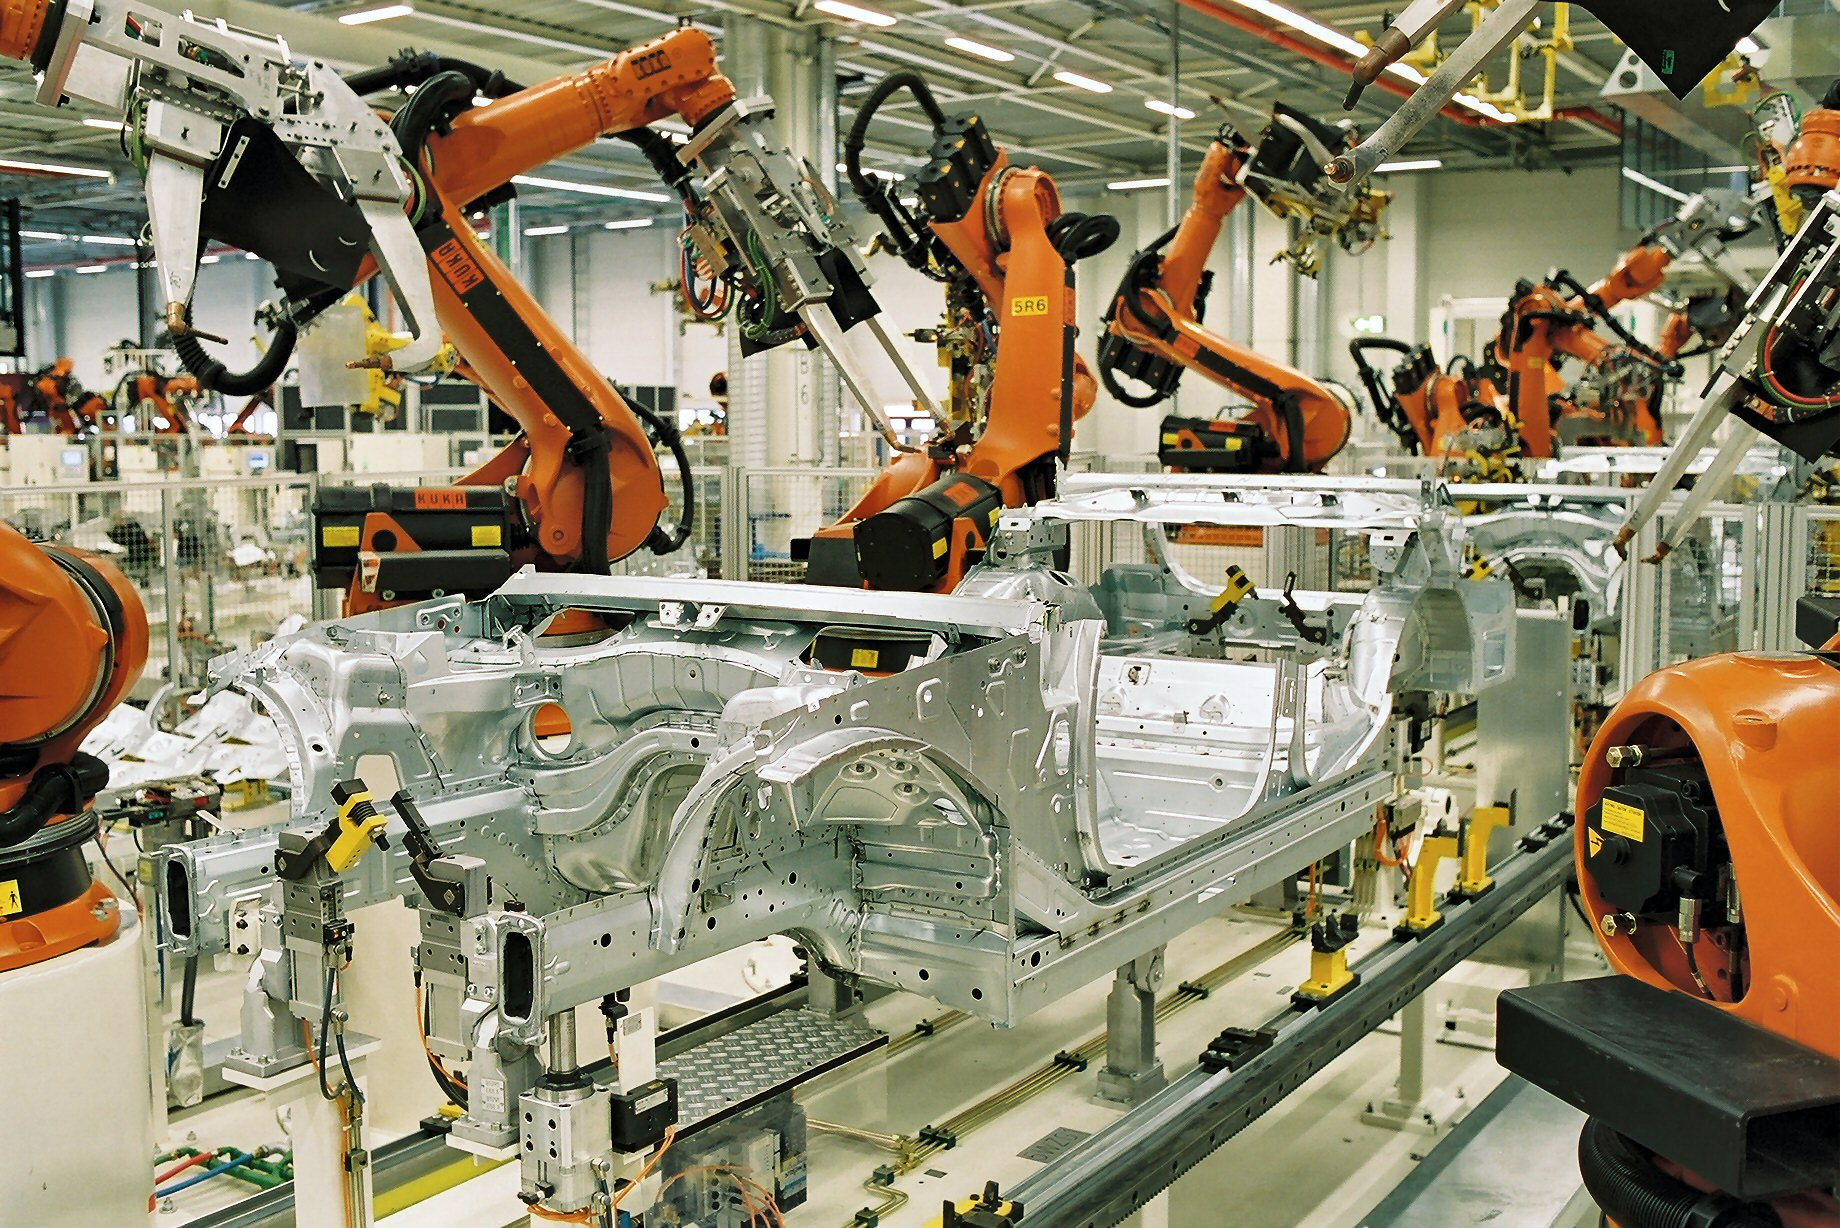
\includegraphics[width=\linewidth,height=3.3cm,keepaspectratio]{../../figures/r23_spot_welding.jpg}\\
\credit{Spot welding of car bodies with KUKA robots. BMW Werk Leipzig, CC BY-SA 2.0 de, via Wikimedia Commons}
\begin{itemize}\small
\item Two copper electrodes squeeze the sheets, a large current melts a small ``nugget''.
\item The heavy \term{weld gun} (50--150 kg) sets the robot size.
\end{itemize}
\column{.5\textwidth}
\centering
\begin{tikzpicture}[x=1cm,y=1cm]
  \fill[mkLight] (-1.8,-.12) rectangle (1.8,0); \fill[mkPale] (-1.8,0) rectangle (1.8,.12);
  \draw[mkGray] (-1.8,-.12) rectangle (1.8,.12);
  \fill[mkOrange!70] (0,0) ellipse (.32 and .1);
  \fill[mkAmber] (-.15,.12) rectangle (.15,1.1); \fill[mkAmber] (-.15,-.12) rectangle (.15,-1.1);
  \draw[-{Latex},mkNavy,thick] (0,1.6) -- (0,1.15) node[pos=0,above,font=\tiny]{force $F\approx$ 3 kN};
  \draw[-{Latex},mkNavy,thick] (0,-1.6) -- (0,-1.15);
  \draw[mkBlue,thick] (.15,.8) -- (1.3,.8) -- (1.3,-.8) -- (.15,-.8);
  \node[draw=mkBlue,fill=white,circle,inner sep=1pt,font=\tiny] at (1.3,0) {$\sim$};
  \node[font=\tiny,right,text=mkBlue] at (1.45,0) {$I\approx$ 10 kA};
  \node[font=\tiny,left,text=mkNavy] at (-.25,.75) {electrode};
  \node[font=\tiny,text=mkOrange] at (-1.0,-.35) {nugget};
  \draw[mkOrange] (-.75,-.3) -- (-.2,-.05);
\end{tikzpicture}
\begin{eqbox}\small
Heat in the joint: $Q = I^2\,R\,t$ \quad (J = A$^2\cdot\Omega\cdot$s)
\end{eqbox}
\footnotesize\textbf{Example:} $I=\SI{10}{kA}$, contact resistance $R=\SI{100}{\micro\ohm}$, $t=\SI{0.2}{s}$:\\
$Q = (10^4)^2\cdot 10^{-4}\cdot 0.2 = \hl{\SI{2000}{J}}$ -- in a 6 mm spot!
\end{columns}
\end{frame}

% ---------------------------------------------------------------------
\begin{frame}[t]{Arc welding: a smooth path at constant speed}
\begin{columns}[T,onlytextwidth]
\column{.52\textwidth}
\centering
\begin{tikzpicture}[x=1cm,y=1cm]
  \fill[mkPale] (-.2,-1.1) rectangle (5.6,-.05); \fill[mkLight] (-.2,.05) rectangle (5.6,1.1);
  \draw[mkGray] (-.2,0) -- (5.6,0);
  \node[font=\tiny,text=mkGray] at (5,.85) {plate 1}; \node[font=\tiny,text=mkGray] at (5,-.85) {plate 2};
  \draw[mkOrange,line width=1pt,domain=0:4.6,samples=150] plot (\x,{.3*sin(\x*360/0.6)});
  \fill[mkBlue] (4.6,0) circle (.08);
  \draw[-{Latex},mkNavy,thick] (4.7,.55) -- (5.4,.55) node[above,font=\tiny]{travel $v$};
  \draw[{Latex}-{Latex},mkMid] (1.35,-.45) -- (1.95,-.45) node[midway,below,font=\tiny]{pitch};
  \draw[{Latex}-{Latex},mkMid] (.1,-.3) -- (.1,.3) node[midway,left,font=\tiny]{width};
  \node[font=\tiny,text=mkOrange,align=center] at (2.4,.75) {weave pattern of the torch};
\end{tikzpicture}
\begin{itemize}\small
\item The torch must follow the seam with a fixed angle and distance.
\item Speed too slow $\to$ burn-through; too fast $\to$ weak seam.
\item Robot uses \term{linear} and \term{circular} moves (4.7), often with \term{weaving}.
\end{itemize}
\column{.45\textwidth}
\begin{defbox}[Worked example -- seam time]
\small
\begin{enumerate}
\item Seam length $L = \SI{1.2}{m} = \SI{1200}{mm}$.
\item Travel speed $v = \SI{8}{mm/s}$.
\item Arc-on time $t = L/v = 1200/8 = \hl{\SI{150}{s}}$.
\item Add air moves and torch cleaning (say \SI{30}{s}) $\to$ \SI{180}{s} per part.
\end{enumerate}
\end{defbox}
\gofurther{Seam tracking (touch sensing, laser line scanners, through-arc sensing) corrects the path when real parts differ from the CAD model.}
\end{columns}
\end{frame}

% ---------------------------------------------------------------------
\begin{frame}[t]{Painting and coating: even layers, no sparks}
\begin{columns}[T,onlytextwidth]
\column{.5\textwidth}
\centering
\begin{tikzpicture}[x=1cm,y=1cm]
  \draw[mkGray,fill=mkLight] (0,0) rectangle (5,2.6);
  \foreach \y/\c in {.35/mkSky,.95/mkMid,1.55/mkSky,2.15/mkMid}{
    \fill[\c,opacity=.35] (0,\y-.45) rectangle (5,\y+.45);
    \draw[-{Latex},mkNavy] (.2,\y) -- (4.8,\y);}
  \draw[{Latex}-{Latex},mkOrange,thick] (5.25,.35) -- (5.25,.95) node[midway,right,font=\tiny]{pitch};
  \draw[{Latex}-{Latex},mkOrange,thick] (-.25,1.1) -- (-.25,2.0) node[midway,left,font=\tiny]{fan width};
  \node[font=\tiny,text=mkNavy] at (2.5,-.25) {overlapping passes (50\,\% overlap)};
\end{tikzpicture}
\begin{itemize}\small
\item Constant gun speed, distance and \hl{overlap} give even thickness.
\item Paint mist is explosive: motors are \term{explosion-proof} (pressurised).
\item Hollow wrist keeps hoses inside the arm.
\end{itemize}
\column{.47\textwidth}
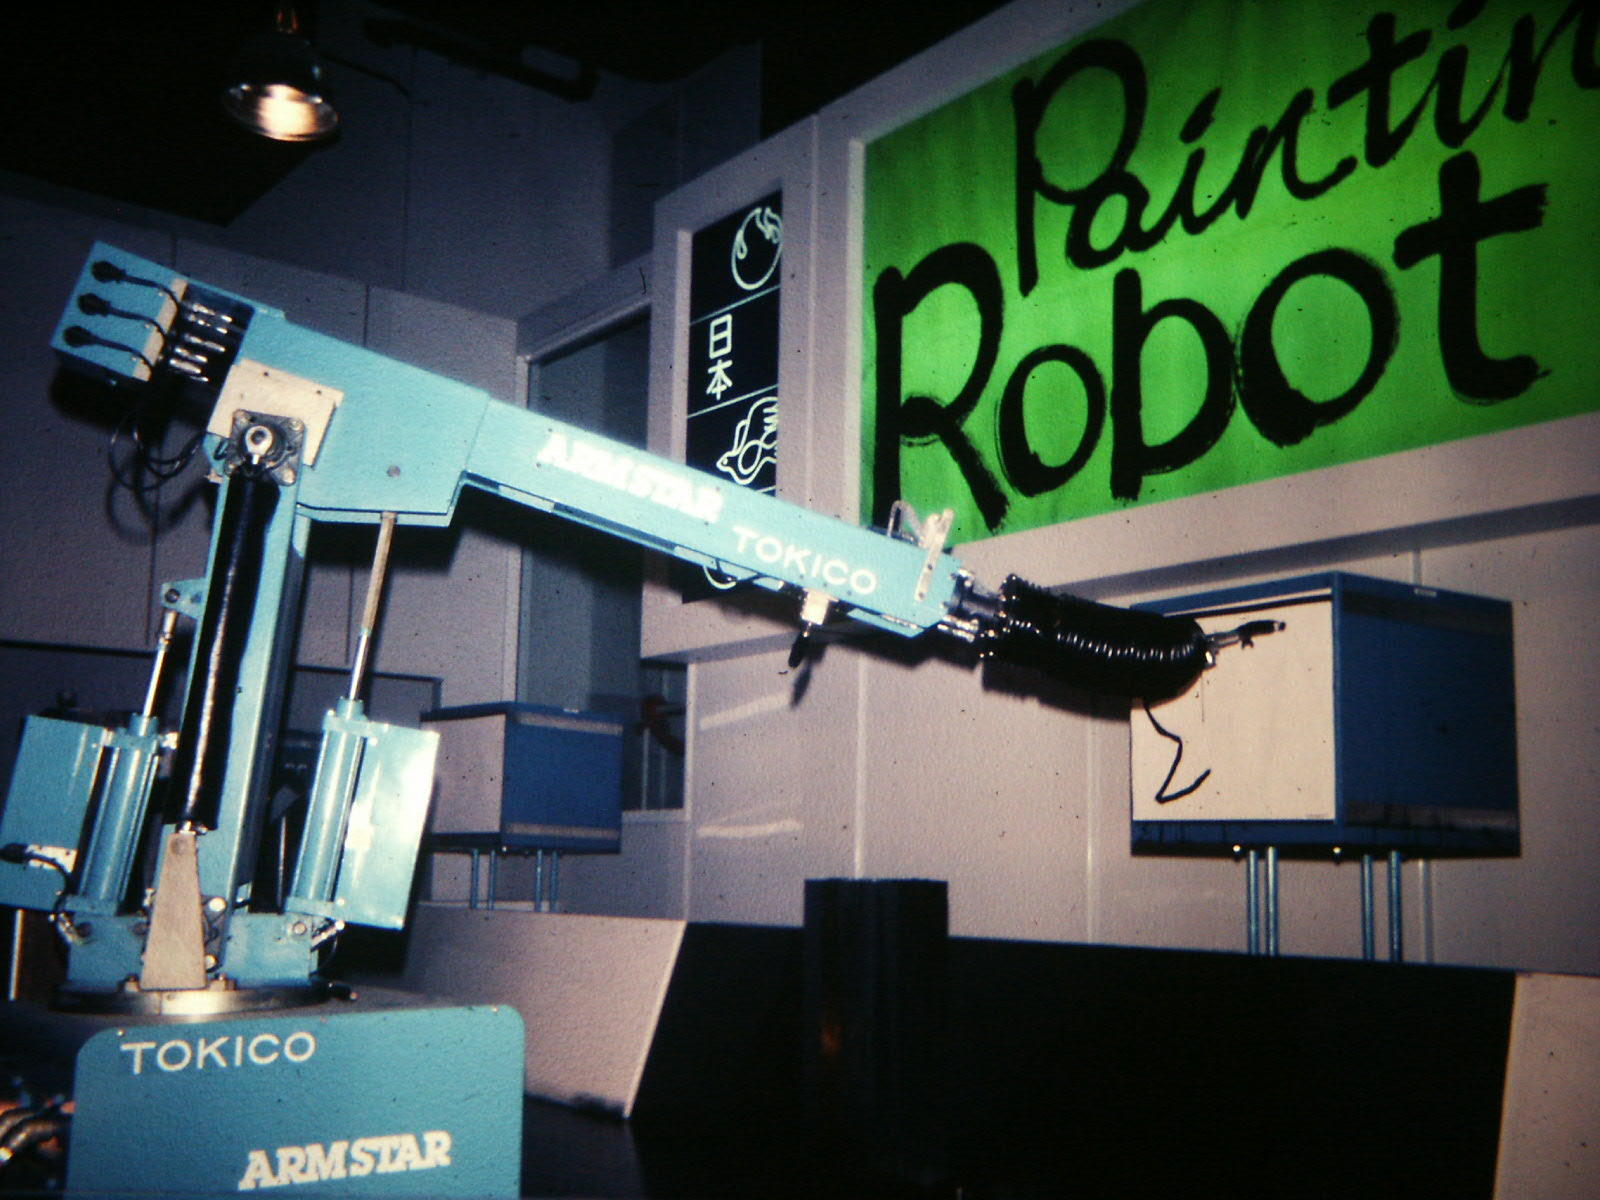
\includegraphics[width=\linewidth,height=2.6cm,keepaspectratio]{../../figures/r23_painting.jpg}\\
\credit{Painting robot (Japan, 1982 World's Fair). Gary Todd, CC0, via Wikimedia Commons}
\begin{defbox}[Worked example -- door panel]
\footnotesize
\begin{enumerate}
\item Fan width \SI{300}{mm}, 50\,\% overlap $\to$ pitch \SI{150}{mm}.
\item Panel height \SI{1.5}{m}: $1500/150 = 10$ passes.
\item Length \SI{2}{m} at \SI{0.5}{m/s}: \SI{4}{s} per pass $\to$ \hl{\SI{40}{s}} + turn-arounds.
\end{enumerate}
\end{defbox}
\end{columns}
\end{frame}

% ---------------------------------------------------------------------
\begin{frame}[t]{Palletising: stacking boxes in stable patterns}
\begin{columns}[T,onlytextwidth]
\column{.5\textwidth}
\centering
\begin{tikzpicture}[x=.55cm,y=.55cm]
  % layer A
  \draw[mkGray] (0,0) rectangle (6,5);
  \foreach \x in {0,2,4}{\foreach \y in {0,1.5}{\draw[fill=mkPale,draw=mkBlue] (\x,\y) rectangle ++(2,1.5);}}
  \foreach \x in {0,1.5,3,4.5}{\draw[fill=mkCream,draw=mkOrange] (\x,3) rectangle ++(1.5,2);}
  \node[font=\tiny,text=mkNavy] at (3,-.5) {layer A};
  % layer B (rotated)
  \begin{scope}[xshift=4cm]
  \draw[mkGray] (0,0) rectangle (6,5);
  \foreach \x in {0,1.5,3,4.5}{\draw[fill=mkCream,draw=mkOrange] (\x,0) rectangle ++(1.5,2);}
  \foreach \x in {0,2,4}{\foreach \y in {2,3.5}{\draw[fill=mkPale,draw=mkBlue] (\x,\y) rectangle ++(2,1.5);}}
  \node[font=\tiny,text=mkNavy] at (3,-.5) {layer B (mirrored)};
  \end{scope}
\end{tikzpicture}
\begin{itemize}\small
\item Alternating layers \hl{interlock} -- like bricks in a wall.
\item Robot program = one pick position + a pattern of place positions (5.5).
\item Typical: 4-axis arm (wrist always vertical), vacuum or fork gripper.
\end{itemize}
\column{.47\textwidth}
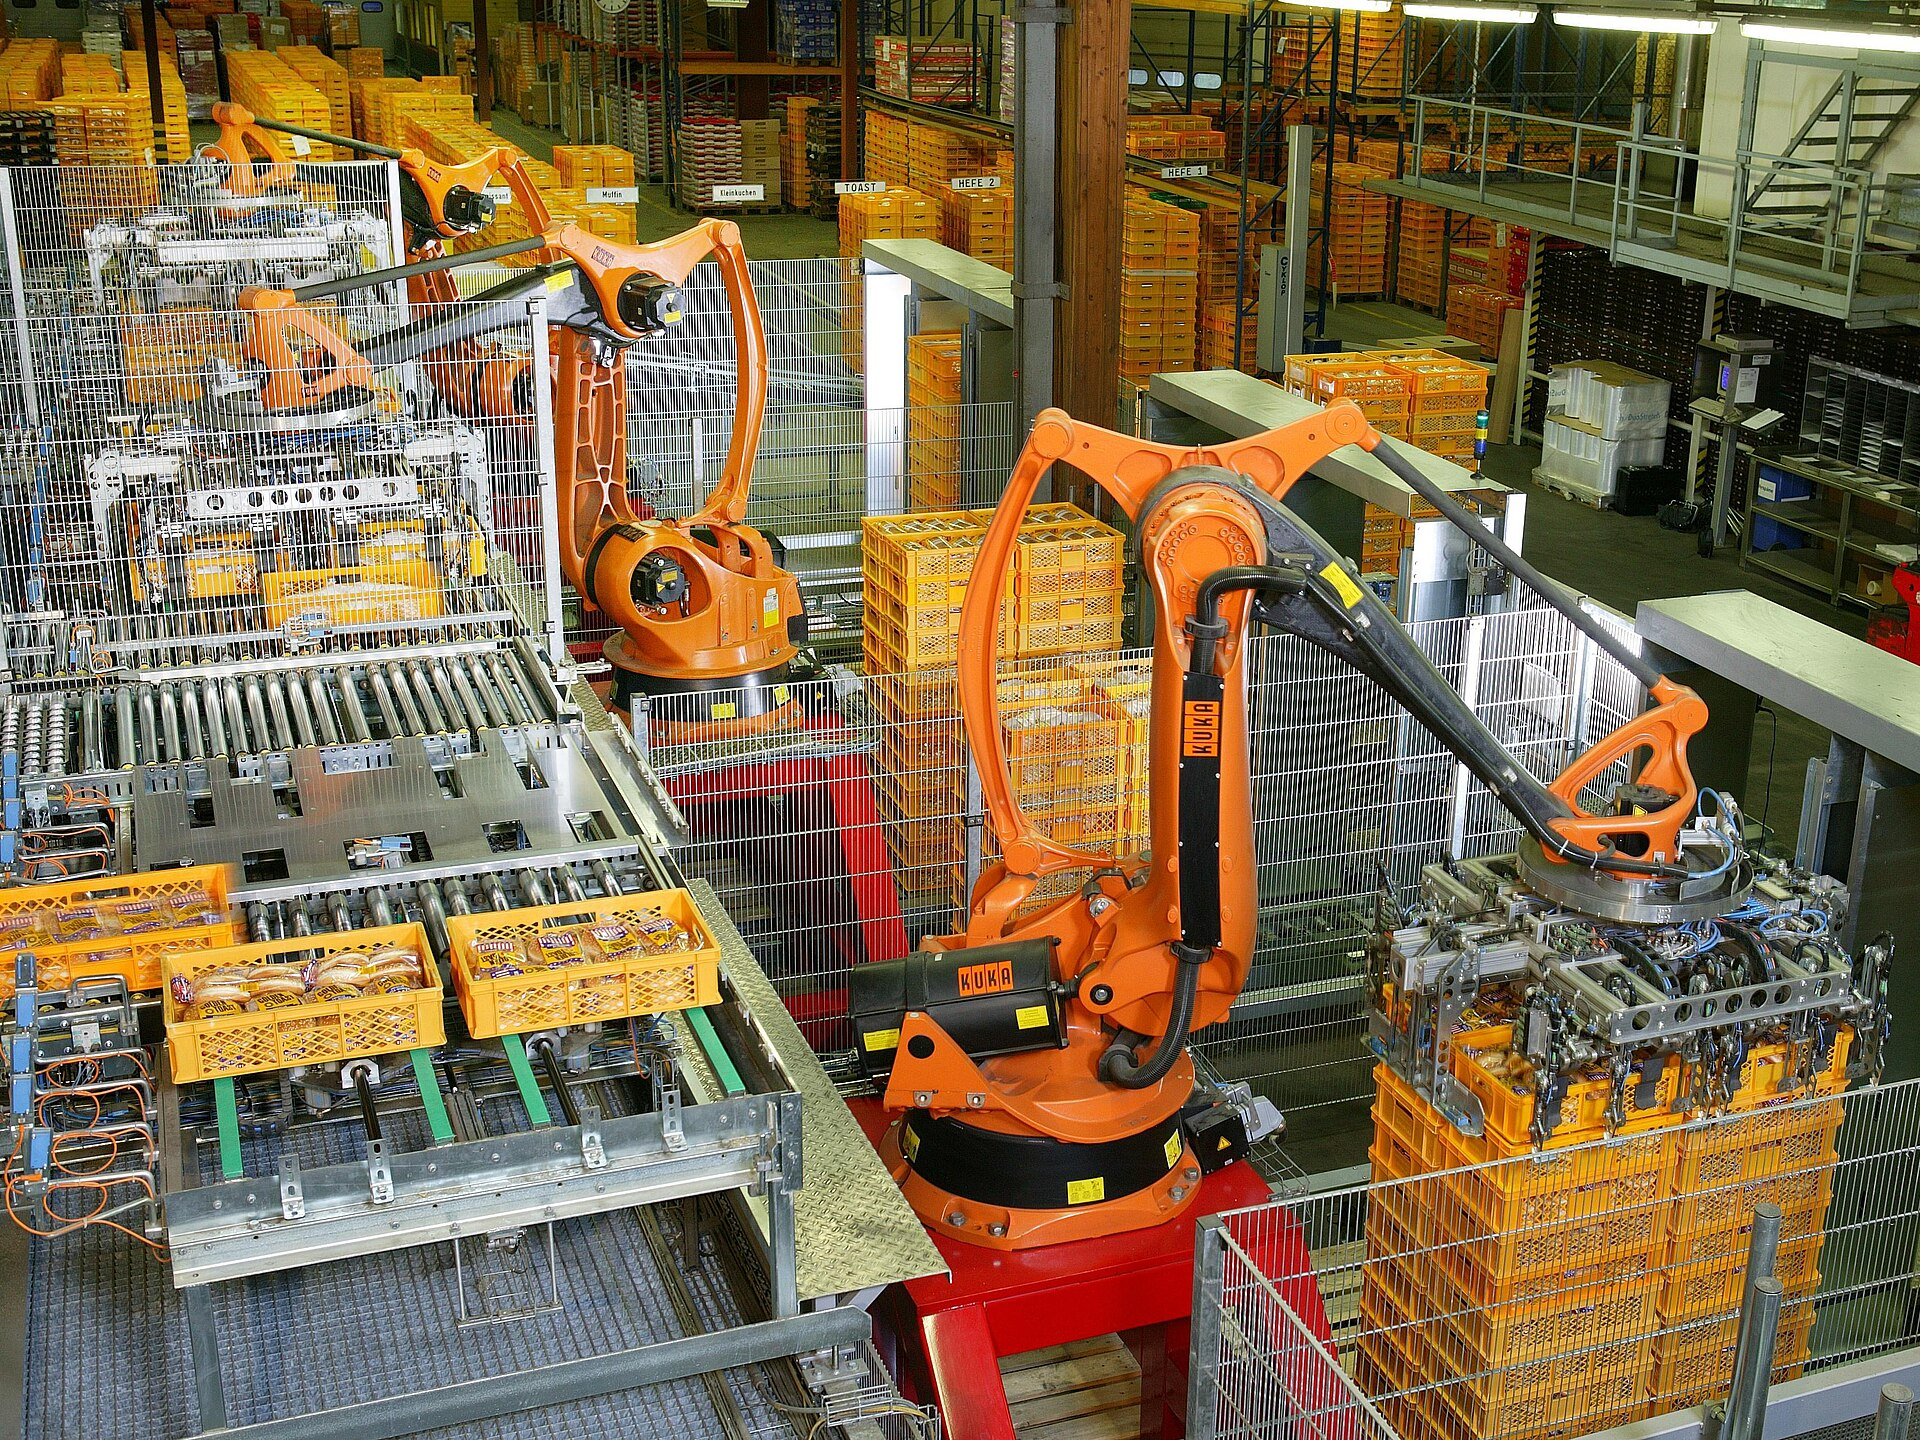
\includegraphics[width=\linewidth,height=3.3cm,keepaspectratio]{../../figures/r23_palletising.jpg}\\
\credit{Robots palletising bread at a bakery. KUKA Roboter GmbH, Bachmann, public domain, via Wikimedia Commons}
\begin{notebox}
\textbf{Rate check:} 12 boxes per minute $\to$ one pick-and-place every \SI{5}{s}.
\end{notebox}
\end{columns}
\end{frame}

% ---------------------------------------------------------------------
\begin{frame}[t]{Machine tending: keep the expensive machine busy}
\begin{columns}[T,onlytextwidth]
\column{.55\textwidth}
\begin{tikzpicture}[x=.023cm,y=1cm]
  \node[font=\scriptsize\bfseries,text=mkNavy,anchor=west] at (0,2.2) {Manual loading};
  \foreach \s in {0,150}{\fill[mkBlue] (\s,1.6) rectangle ++(90,.35); \fill[mkGray!40] (\s+90,1.6) rectangle ++(60,.35);}
  \node[font=\scriptsize\bfseries,text=mkNavy,anchor=west] at (0,1.15) {Robot loading};
  \foreach \s in {0,105,210}{\fill[mkBlue] (\s,.55) rectangle ++(90,.35); \fill[mkOrange] (\s+90,.55) rectangle ++(15,.35);}
  \draw[mkGray,-{Latex}] (0,.3) -- (310,.3) node[right,font=\tiny]{$t$ (s)};
  \foreach \t in {0,100,200,300}{\draw[mkGray] (\t,.25)--(\t,.35); \node[font=\tiny,text=mkGray] at (\t,.1) {\t};}
  \fill[mkBlue] (0,-.3) rectangle ++(8,.18); \node[font=\tiny,anchor=west] at (9,-.21) {machining 90 s};
  \fill[mkGray!40] (95,-.3) rectangle ++(8,.18); \node[font=\tiny,anchor=west] at (104,-.21) {manual load 60 s};
  \fill[mkOrange] (200,-.3) rectangle ++(8,.18); \node[font=\tiny,anchor=west] at (209,-.21) {robot load 15 s};
\end{tikzpicture}
\begin{eqbox}\small
Machine utilisation $U = \dfrac{t_\text{machining}}{t_\text{machining}+t_\text{load}}$
\end{eqbox}
\column{.42\textwidth}
\begin{itemize}\small
\item Robot opens the door, unloads the finished part, loads a raw part, closes the door, starts the cycle.
\item Runs nights and weekends (``lights-out'').
\end{itemize}
\begin{defbox}[Worked example]
\footnotesize
\begin{enumerate}
\item Manual: $U = 90/(90+60) = 60\,\%$.
\item Robot: $U = 90/(90+15) = \hl{86\,\%}$.
\item Same machine, $+43\,\%$ more parts.
\end{enumerate}
\end{defbox}
\end{columns}
\end{frame}

% ---------------------------------------------------------------------
\begin{frame}[t]{Assembly and pick-and-place: speed and gentle precision}
\begin{columns}[T,onlytextwidth]
\column{.48\textwidth}
\centering
\begin{tikzpicture}[x=1cm,y=1cm]
  % hole block
  \fill[mkLight] (-1.6,-1.6) rectangle (-.35,0); \fill[mkLight] (.35,-1.6) rectangle (1.6,0);
  \fill[mkLight] (-.35,-1.6) rectangle (.35,-1.5);
  \draw[mkGray] (-1.6,0) -- (-.5,0) -- (-.35,-.15) -- (-.35,-1.5) -- (.35,-1.5) -- (.35,-.15) -- (.5,0) -- (1.6,0);
  % peg slightly offset
  \fill[mkBlue!60] (-.2,.05) rectangle (.42,1.3);
  \draw[mkNavy] (-.2,.05) rectangle (.42,1.3);
  \draw[-{Latex},mkOrange,thick] (.11,1.75) -- (.11,1.35) node[pos=0,above,font=\tiny]{push};
  \node[font=\tiny,text=mkOrange,align=left,anchor=west] at (.65,.05) {chamfer guides\\the peg in};
  \draw[mkOrange] (.6,.05) -- (.45,-.05);
  \node[font=\tiny,text=mkGray] at (0,-1.85) {peg-in-hole: clearance $\approx$ 0.01--0.05 mm};
\end{tikzpicture}
\begin{itemize}\small
\item Assembly needs \hl{compliance}: a little ``give'' so small misalignments don't jam.
\item Chamfers, compliant wrists or force control (2.9) help.
\end{itemize}
\column{.49\textwidth}
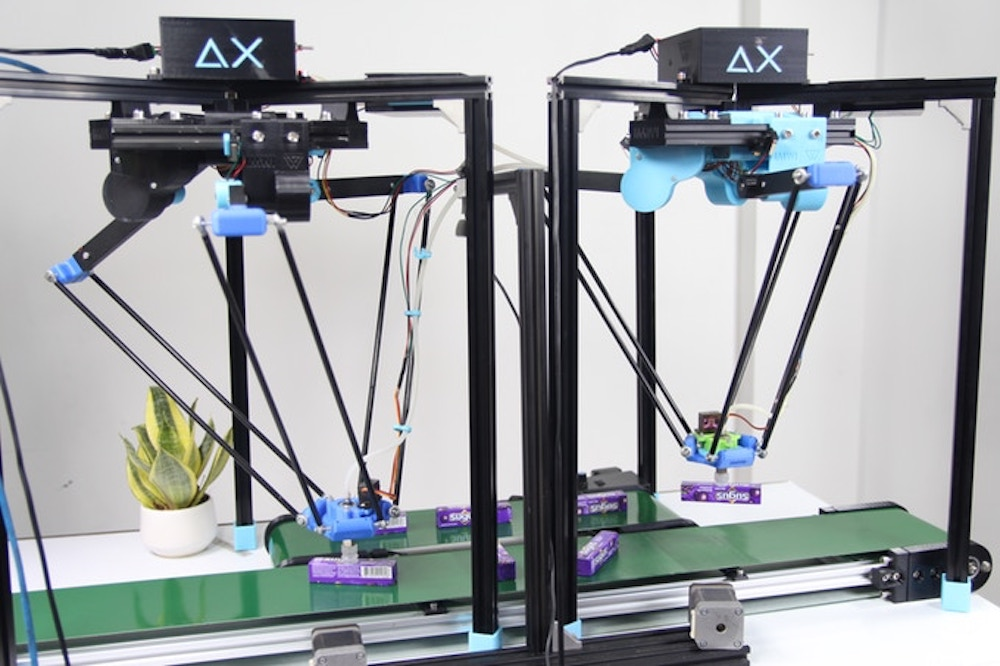
\includegraphics[width=\linewidth,height=2.7cm,keepaspectratio]{../../figures/r23_delta.jpg}\\
\credit{Delta robots picking from a conveyor. Trungdoanhong, CC BY-SA 4.0, via Wikimedia Commons}
\begin{itemize}\small
\item \term{Pick-and-place}: light parts, very fast -- delta and SCARA robots.
\item 120 picks/min $\to$ \hl{\SI{0.5}{s}} per pick incl.\ up, across, down, release.
\end{itemize}
\gofurther{A remote-centre-compliance (RCC) wrist lets the peg rotate about its tip, so contact forces straighten it.}
\end{columns}
\end{frame}

% ---------------------------------------------------------------------
\begin{frame}[t]{Check your understanding -- 5.2}
\vspace{4mm}
\begin{keybox}[Check your understanding]
\large
\begin{enumerate}
\item Why is the robot for spot welding usually much bigger than the robot for arc welding on the same car?\\[3mm]
\item A robot always returns within $\pm$0.03 mm of a taught point, but misses a CAD-calculated point by 0.8 mm. Which property is good, which is poor?\\[3mm]
\item A CNC cycle is 60 s; manual loading takes 40 s, robot loading 10 s. Calculate both machine utilisations.
\end{enumerate}
\end{keybox}
\vfill
\centering\small\color{mkGray} Discuss with your neighbour for 2 minutes.
\end{frame}

% ---------------------------------------------------------------------
\begin{frame}{Summary 5.2 -- Industrial robot applications}
\begin{columns}[T,onlytextwidth]
\column{.55\textwidth}
\begin{keybox}[Key take-aways]
\small
\begin{itemize}
\item About half of robots do handling; welding is next.
\item The process sets the robot: payload, reach, path quality, speed, environment.
\item Spot welding: heavy gun; arc welding and painting: smooth, constant-speed paths.
\item Palletising and pick-and-place: patterns and speed; assembly: compliance.
\item Robots are more repeatable than accurate.
\end{itemize}
\end{keybox}
\column{.42\textwidth}
\begin{defbox}[Key terms]
\small
\textbf{Payload} -- mass the wrist may carry.\\
\textbf{Reach} -- max.\ wrist distance.\\
\textbf{Repeatability} -- return to a taught point.\\
\textbf{Accuracy} -- hit a calculated point.\\
\textbf{Machine tending} -- loading a machine.\\
\textbf{Compliance} -- controlled ``give''.
\end{defbox}
\end{columns}
\end{frame}

% =====================================================================
\section{5.3 Robotic Work-Cell Design}
% =====================================================================

\begin{frame}[t]{What is a robotic work-cell?}
\begin{columns}[T,onlytextwidth]
\column{.55\textwidth}
\centering
\begin{tikzpicture}[x=1cm,y=1cm]
  \draw[mkOrange,line width=1.2pt,dash pattern=on 3pt off 2pt] (-3,-2.1) rectangle (3.3,2.1);
  \node[font=\tiny,text=mkOrange,anchor=south west] at (-3,2.1) {safety fence};
  \fill[mkPale] (0,0) circle (1.9); \draw[mkSky,dashed] (0,0) circle (1.9);
  \fill[mkBlue] (0,0) circle (.32); \node[font=\tiny,white] at (0,0) {robot};
  \draw[fill=mkLight,draw=mkNavy] (-2.8,-.7) rectangle (-1.6,.7); \node[font=\tiny,align=center] at (-2.2,0) {CNC\\lathe};
  \draw[fill=mkCream,draw=mkOrange] (1.1,.9) rectangle (2.0,1.6); \node[font=\tiny,align=center] at (1.55,1.25) {check\\station};
  \draw[fill=mkLight,draw=mkNavy] (1.3,-1.7) rectangle (2.5,-.6); \node[font=\tiny] at (1.9,-1.15) {pallet};
  \draw[fill=mkGray!30,draw=mkGray] (-1.2,1.3) rectangle (.6,1.75); \node[font=\tiny] at (-.3,1.52) {conveyor in};
  \draw[fill=white,draw=mkNavy] (3.5,.6) rectangle (4.5,1.6); \node[font=\tiny,align=center] at (4,1.1) {robot\\ctrl.};
  \draw[fill=white,draw=mkNavy] (3.5,-.4) rectangle (4.5,.4); \node[font=\tiny] at (4,0) {PLC};
  \draw[fill=mkOrange!30,draw=mkOrange] (3.5,-1.6) rectangle (4.5,-.8); \node[font=\tiny,align=center] at (4,-1.2) {HMI};
  \draw[mkMid,thick] (3.3,-1.7) -- (3.3,-.9); \node[font=\tiny,text=mkMid,rotate=90] at (3.15,-1.3) {door};
\end{tikzpicture}
\column{.42\textwidth}
\begin{itemize}\small
\item \term{Work-cell}: robot + everything it needs to do one job on its own.
\item Robot, \term{end-of-arm tooling} (EOAT), fixtures, feeders/conveyors, process equipment.
\item Control: robot controller, \term{PLC}, operator panel (\term{HMI}).
\item Guarding: fence, interlocked door, light curtain (W2D4).
\end{itemize}
\begin{keybox}[Analogy]
A kitchen: the cook (robot) is only fast if pots, knives and fridge are all within arm's reach.
\end{keybox}
\end{columns}
\end{frame}

% ---------------------------------------------------------------------
\begin{frame}[t]{Cell layouts: three common patterns}
\centering
\begin{tikzpicture}[x=1cm,y=1cm]
  % 1 robot-centred
  \begin{scope}[xshift=0cm]
    \fill[mkPale] (0,0) circle (1.2); \fill[mkBlue] (0,0) circle (.22);
    \foreach \a/\t in {0/A,90/B,180/C,270/D}{\draw[fill=mkCream,draw=mkOrange] (\a:1.05) ++(-.25,-.2) rectangle ++(.5,.4); \node[font=\tiny] at (\a:1.05) {\t};}
    \node[font=\scriptsize\bfseries,text=mkNavy] at (0,-1.7) {robot-centred};
    \node[font=\tiny,text=mkGray,align=center] at (0,-2.2) {stations around one robot};
  \end{scope}
  % 2 in-line
  \begin{scope}[xshift=4.6cm]
    \fill[mkGray!30] (-2,-.15) rectangle (2,.15); \draw[-{Latex},mkNavy] (-1.9,0) -- (1.9,0);
    \foreach \x in {-1.3,0,1.3}{\fill[mkPale] (\x,.65) circle (.45); \fill[mkBlue] (\x,.65) circle (.16);}
    \foreach \x in {-1.3,0,1.3}{\fill[mkPale] (\x,-.65) circle (.45); \fill[mkMid] (\x,-.65) circle (.16);}
    \node[font=\scriptsize\bfseries,text=mkNavy] at (0,-1.7) {in-line};
    \node[font=\tiny,text=mkGray,align=center] at (0,-2.2) {robots along a conveyor (car body line)};
  \end{scope}
  % 3 mobile / track
  \begin{scope}[xshift=9.4cm]
    \fill[mkGray!30] (-1.9,-.08) rectangle (1.9,.08);
    \draw[fill=mkBlue] (-.4,-.2) rectangle (.0,.2);
    \draw[{Latex}-{Latex},mkOrange,thick] (-1.6,.4) -- (1.6,.4);
    \foreach \x in {-1.4,-.4,.6,1.6}{\draw[fill=mkLight,draw=mkNavy] (\x-.35,-1.1) rectangle (\x+.05,-.6);}
    \node[font=\scriptsize\bfseries,text=mkNavy] at (0,-1.7) {robot on a linear track};
    \node[font=\tiny,text=mkGray,align=center] at (0,-2.2) {one robot serves several machines};
  \end{scope}
\end{tikzpicture}
\vspace{2mm}
\begin{columns}[T,onlytextwidth]
\column{.5\textwidth}
\begin{itemize}\small
\item \textbf{Robot-centred:} compact, cheap, one robot = bottleneck.
\item \textbf{In-line:} high volume; each robot does a small piece of work.
\end{itemize}
\column{.47\textwidth}
\begin{itemize}\small
\item \textbf{Track / gantry / AMR:} extends reach; adds an extra (7th) axis.
\item Choose by volume, part size and floor space.
\end{itemize}
\end{columns}
\end{frame}

% ---------------------------------------------------------------------
\begin{frame}[t]{Reach check: is every station inside the comfort zone?}
\begin{columns}[T,onlytextwidth]
\column{.48\textwidth}
\centering
\begin{tikzpicture}[x=1.6cm,y=1.6cm]
  \fill[mkPale] (0,0) circle (1.4); \fill[mkCream] (0,0) circle (1.19); \fill[mkPale] (0,0) circle (.42); \fill[white] (0,0) circle (.25);
  \draw[mkSky] (0,0) circle (1.4); \draw[mkOrange,dashed] (0,0) circle (1.19); \draw[mkOrange,dashed] (0,0) circle (.42);
  \fill[mkBlue] (0,0) circle (.08);
  \draw[mkGray,-{Latex}] (-1.6,0) -- (1.6,0) node[right,font=\tiny]{$x$ (m)};
  \draw[mkGray,-{Latex}] (0,-1.5) -- (0,1.6) node[above,font=\tiny]{$y$};
  \draw[fill=mkNavy] (1.0,.6) circle (.05) node[above right,font=\tiny]{P (1.0, 0.6)};
  \draw[mkNavy,dashed] (0,0) -- (1.0,.6);
  \draw[fill=mkRed] (-.9,-1.1) circle (.05) node[left,font=\tiny,text=mkRed]{Q};
  \node[font=\tiny,text=mkOrange] at (-.95,.95) {85\,\%};
  \node[font=\tiny,text=mkSky] at (0,1.5) {max.\ reach 1.4 m};
\end{tikzpicture}
\column{.5\textwidth}
\begin{itemize}\small
\item Near full reach the arm is stretched (close to a \term{singularity}, slow, little stiffness).
\item Too close to the base the arm folds onto itself.
\item Rule of thumb: place stations at \hl{30--85\,\%} of max.\ reach, at a good height.
\end{itemize}
\begin{defbox}[Worked example]
\footnotesize
\begin{enumerate}
\item Point P: $r = \sqrt{1.0^2+0.6^2} = \SI{1.17}{m}$.
\item Ratio: $1.17/1.4 = 83\,\%$ $\to$ OK, but at the limit.
\item Point Q $(-0.9,-1.1)$: $r = \SI{1.42}{m} > \SI{1.4}{m}$ $\to$ \hl{unreachable}; move the station.
\end{enumerate}
\end{defbox}
\gofurther{Reach is not enough: the tool also needs the right \emph{orientation} at that point. Check it in simulation (5.5).}
\end{columns}
\end{frame}

% ---------------------------------------------------------------------
\begin{frame}[t]{Cycle time: where do the seconds go?}
\begin{columns}[T,onlytextwidth]
\column{.55\textwidth}
\begin{tikzpicture}
\begin{axis}[mkplot, xbar stacked, width=7.8cm, height=4.4cm, xmin=0, xmax=14,
  symbolic y coords={improved,original}, ytick=data, y tick label style={font=\scriptsize,text=mkNavy},
  xlabel={time per part (s)}, bar width=14pt, grid=none, enlarge y limits=.5,
  legend style={at={(.5,1.04)},anchor=south,legend columns=5}]
\addplot[fill=mkBlue,draw=white] coordinates {(5.0,original) (3.6,improved)};
\addplot[fill=mkSky,draw=white] coordinates {(2.0,original) (1.2,improved)};
\addplot[fill=mkOrange,draw=white] coordinates {(3.0,original) (3.0,improved)};
\addplot[fill=mkGray!50,draw=white] coordinates {(2.0,original) (0.2,improved)};
\legend{robot moves,grip/release,process (check),waiting}
\end{axis}
\end{tikzpicture}
\begin{itemize}\small
\item \term{Cycle time}: time between two finished parts leaving the cell.
\item Biggest savings usually come from \hl{removing waiting}, not from a faster robot.
\end{itemize}
\column{.42\textwidth}
\begin{defbox}[How the 12 s became 8 s]
\small
\begin{itemize}
\item Shorter, blended moves (5.5): $-1.4$ s.
\item Gripper valve closer to the tool: $-0.8$ s.
\item Next part waits ready in a buffer: $-1.8$ s.
\end{itemize}
\end{defbox}
\begin{notebox}
\textbf{Parallel work}: while the CNC machines part $n$, the robot checks and stacks part $n-1$.
\end{notebox}
\end{columns}
\end{frame}

% ---------------------------------------------------------------------
\begin{frame}[t]{Takt time and throughput: is the cell fast enough?}
\begin{columns}[T,onlytextwidth]
\column{.48\textwidth}
\begin{tikzpicture}
\begin{axis}[mkplot, width=6.6cm, height=4.6cm, xmin=4, xmax=20, ymin=0, ymax=950,
  xlabel={cycle time $t_c$ (s)}, ylabel={parts per hour}]
\addplot[mkBlue,thick,domain=4:20,samples=60] {3600/x};
\addplot[mkOrange,dashed,thick] coordinates {(4,360) (20,360)};
\addplot[only marks,mark=*,mkOrange,mark size=1.6pt] coordinates {(10,360)};
\addplot[only marks,mark=*,mkRed,mark size=1.6pt] coordinates {(12,300)};
\node[font=\tiny,text=mkOrange,anchor=south west] at (axis cs:12.5,370) {demand 360/h};
\node[font=\tiny,text=mkRed,anchor=south west] at (axis cs:5,150) {12 s $\to$ 300/h};
\end{axis}
\end{tikzpicture}
\column{.5\textwidth}
\begin{eqbox}\small
Takt time $\;t_\text{takt} = \dfrac{\text{available time}}{\text{demand}}$; \quad need $t_c \le t_\text{takt}$
\end{eqbox}
\begin{defbox}[Worked example]
\footnotesize
\begin{enumerate}
\item Shift: \SI{7.5}{h} $= \SI{27000}{s}$; demand 2700 parts/shift.
\item $t_\text{takt} = 27000/2700 = \SI{10}{s}$ (360 parts/h).
\item Cell cycle $t_c = \SI{12}{s}$ $\to$ $3600/12 = 300$ parts/h. \hl{Too slow!}
\item Fix: shorten the cycle to $\le$ 10 s (previous slide) or add a second robot.
\end{enumerate}
\end{defbox}
\small \term{Takt} (German: beat) = the rhythm the customer demands.
\end{columns}
\end{frame}

% ---------------------------------------------------------------------
\begin{frame}[t]{Estimating a robot move time}
\begin{columns}[T,onlytextwidth]
\column{.5\textwidth}
\begin{tikzpicture}
\begin{axis}[mkplot, width=6.8cm, height=4.6cm, xmin=0, xmax=1.6, ymin=0, ymax=1.1,
  xlabel={distance $d$ (m)}, ylabel={move time $t$ (s)}, legend pos=south east]
\addplot[mkSky,thick,dashed,domain=0:0.4,samples=40] {2*sqrt(x/10)};
\addplot[mkBlue,thick,domain=0.4:1.6,samples=20] {x/2+0.2};
\addplot[only marks,mark=*,mkOrange,mark size=1.6pt] coordinates {(1.0,0.7)};
\draw[mkGray,dotted] (axis cs:0.4,0) -- (axis cs:0.4,0.4);
\legend{triangular (never reaches $v$),trapezoidal}
\node[font=\tiny,text=mkOrange,anchor=north west] at (axis cs:1.0,0.68) {1 m $\to$ 0.7 s};
\end{axis}
\end{tikzpicture}
\column{.48\textwidth}
\small Remember the trapezoidal velocity profile (4.7): accelerate, cruise, brake.
\begin{eqbox}\small
$t = \dfrac{d}{v_\text{max}} + \dfrac{v_\text{max}}{a}$ \quad if $d \ge v_\text{max}^2/a$
\end{eqbox}
\begin{defbox}[Worked example]
\footnotesize
\begin{enumerate}
\item $v_\text{max}=\SI{2}{m/s}$, $a=\SI{10}{m/s^2}$, $d=\SI{1}{m}$.
\item Check: $v^2/a = 0.4\,\text{m} \le 1\,\text{m}$ $\to$ trapezoid.
\item $t = 1/2 + 2/10 = \hl{\SI{0.7}{s}}$.
\end{enumerate}
\end{defbox}
\footnotesize Short moves are dominated by acceleration: halving the distance does \emph{not} halve the time.
\end{columns}
\end{frame}

% ---------------------------------------------------------------------
\begin{frame}[t]{End-of-arm tooling (EOAT) and grip force}
\begin{columns}[T,onlytextwidth]
\column{.45\textwidth}
\centering
\begin{tikzpicture}[x=1cm,y=1cm]
  \fill[mkGray!40] (-1.0,1.4) rectangle (1.0,1.9); \node[font=\tiny] at (0,1.65) {gripper body};
  \fill[mkMid] (-.75,-.4) rectangle (-.5,1.4); \fill[mkMid] (.5,-.4) rectangle (.75,1.4);
  \fill[mkAmber] (-.5,-.3) rectangle (.5,.9); \node[font=\tiny] at (0,.3) {part $m$};
  \draw[-{Latex},mkOrange,thick] (-1.5,.3) -- (-.78,.3) node[pos=0,left,font=\tiny]{$F$};
  \draw[-{Latex},mkOrange,thick] (1.5,.3) -- (.78,.3) node[pos=0,right,font=\tiny]{$F$};
  \draw[-{Latex},mkBlue,thick] (-.42,0) -- (-.42,.6) node[above,font=\tiny]{$\mu F$};
  \draw[-{Latex},mkBlue,thick] (.42,0) -- (.42,.6);
  \draw[-{Latex},mkNavy,thick] (0,-.35) -- (0,-1.1) node[below,font=\tiny]{$m(g+a)$};
\end{tikzpicture}
\begin{eqbox}\small
$n\,\mu\,F \;\ge\; m\,(g+a)\,S$
\end{eqbox}
\footnotesize $n$ friction surfaces, $\mu$ friction coeff., $F$ finger force (N), $a$ upward accel., $S$ safety factor.
\column{.52\textwidth}
\begin{itemize}\small
\item EOAT: the robot's ``hand'' -- fingers, vacuum cups, magnets, tools (W1D2).
\item Usually custom-made for each part; often 10--30\,\% of cell cost.
\item \term{Tool changer}: swap grippers automatically.
\end{itemize}
\begin{defbox}[Worked example]
\footnotesize
\begin{enumerate}
\item $m=\SI{2}{kg}$, $a=\SI{5}{m/s^2}$, $\mu=0.3$, $n=2$, $S=2$.
\item Needed friction: $2\cdot(9.81+5)\cdot 2 = \SI{59}{N}$.
\item $F \ge 59/(2\cdot0.3) = \hl{\SI{99}{N}} \approx \SI{100}{N}$ per finger.
\end{enumerate}
\end{defbox}
\footnotesize Friction grip is weak: shaped fingers that ``cradle'' the part are much safer.
\end{columns}
\end{frame}

% ---------------------------------------------------------------------
\begin{frame}[t]{Fixtures and part presentation: the 3-2-1 rule}
\begin{columns}[T,onlytextwidth]
\column{.5\textwidth}
\centering
\begin{tikzpicture}[x=1cm,y=1cm]
  \draw[mkNavy,fill=mkPale,thick] (0,0) rectangle (3.4,2.2);
  \node[font=\tiny,text=mkNavy] at (1.7,.9) {part (top view)};
  \foreach \p in {(.5,.45),(2.9,.45),(1.7,1.8)}{\draw[mkOrange,fill=mkOrange!40,thick] \p circle (.13);}
  \foreach \y in {.5,1.7}{\fill[mkBlue] (0,\y) -- (-.3,\y+.18) -- (-.3,\y-.18) -- cycle;}
  \fill[mkGreen] (1.7,0) -- (1.52,-.3) -- (1.88,-.3) -- cycle;
  \draw[-{Latex},mkGray,thick] (4.1,1.1) -- (3.5,1.1) node[pos=0,right,font=\tiny]{clamp};
  \draw[-{Latex},mkGray,thick] (1.7,2.9) -- (1.7,2.3) node[pos=0,above,font=\tiny]{clamp};
  \node[font=\tiny,text=mkOrange,anchor=north] at (1.7,1.55) {3 support pins below};
  \node[font=\tiny,text=mkBlue,anchor=east] at (-.35,1.1) {2 side};
  \node[font=\tiny,text=mkGreen,anchor=north] at (1.7,-.32) {1 end stop};
\end{tikzpicture}
\begin{itemize}\small
\item 3 + 2 + 1 points fix all 6 DOF of a rigid part (4.1).
\item Then a clamp pushes the part against them.
\end{itemize}
\column{.47\textwidth}
\begin{itemize}\small
\item The robot repeats blindly: the part must be \hl{in the same place every time}.
\item \term{Fixture}: holds the part in a defined position.
\item \term{Feeders}: bowl feeder, trays, conveyor with end stop.
\item No fixture? Then a \term{vision} system must find the part (W2D5).
\end{itemize}
\begin{keybox}[Take-away]
Good fixtures make simple robot programs; bad fixtures cause most cell stops.
\end{keybox}
\end{columns}
\end{frame}

% ---------------------------------------------------------------------
\begin{frame}[t]{Check your understanding -- 5.3}
\vspace{4mm}
\begin{keybox}[Check your understanding]
\large
\begin{enumerate}
\item A station is at $(1.2, 0.9)$ m from a robot with \SI{1.6}{m} reach. Is it in the comfort zone?\\[3mm]
\item Demand is 1800 parts in a \SI{7.5}{h} shift. What is the takt time? Is a 14 s cycle enough?\\[3mm]
\item Why does halving a short robot move not halve its time?
\end{enumerate}
\end{keybox}
\vfill
\centering\small\color{mkGray} Discuss with your neighbour for 2 minutes.
\end{frame}

% ---------------------------------------------------------------------
\begin{frame}{Summary 5.3 -- Work-cell design}
\begin{columns}[T,onlytextwidth]
\column{.55\textwidth}
\begin{keybox}[Key take-aways]
\small
\begin{itemize}
\item A cell = robot + EOAT + fixtures + feeders + controls + guarding.
\item Place stations at about 30--85\,\% of reach, with the right orientation.
\item Cycle time must be $\le$ takt time; remove waiting first.
\item Move time $\approx d/v + v/a$ for long moves.
\item Grip force from $n\mu F \ge m(g+a)S$; fixtures use the 3-2-1 rule.
\end{itemize}
\end{keybox}
\column{.42\textwidth}
\begin{defbox}[Key terms]
\small
\textbf{Work-cell} -- self-contained robot station.\\
\textbf{EOAT} -- end-of-arm tooling.\\
\textbf{Cycle time} -- time per finished part.\\
\textbf{Takt time} -- time per part the demand allows.\\
\textbf{Fixture} -- holds the part in place.\\
\textbf{HMI} -- operator screen/panel.
\end{defbox}
\end{columns}
\end{frame}

% =====================================================================
\section{5.4 PLCs and Automation Control}
% =====================================================================

\begin{frame}[t]{Why PLCs? From relay cabinets to a rugged computer}
\begin{columns}[T,onlytextwidth]
\column{.5\textwidth}
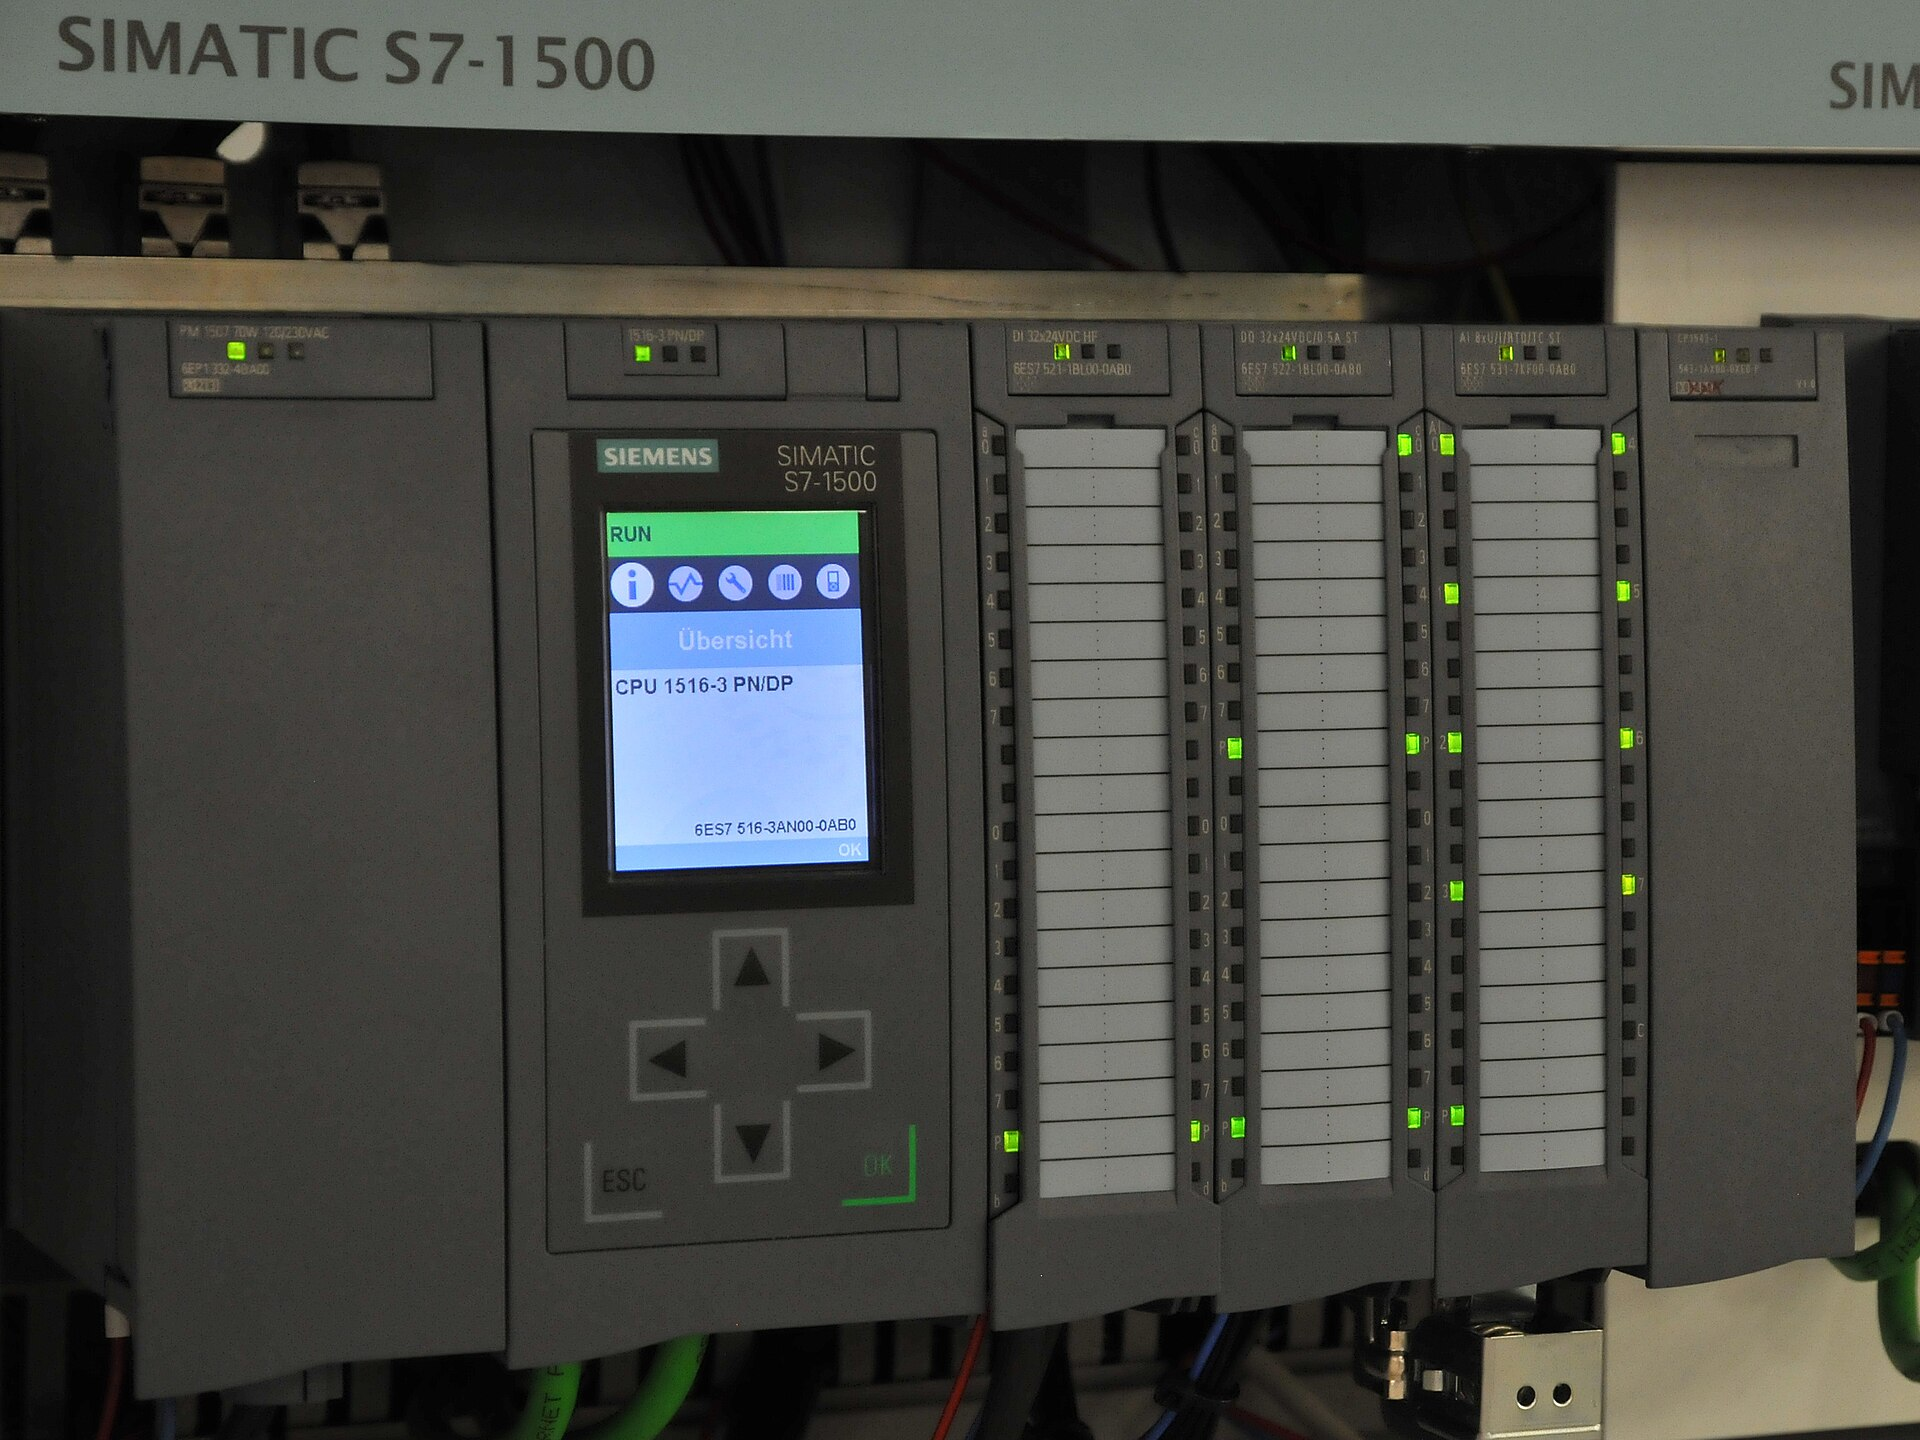
\includegraphics[width=\linewidth,height=3.4cm,keepaspectratio]{../../figures/r23_plc.jpg}\\
\credit{Modular PLC (CPU + I/O modules). Palatinatian, CC BY 3.0, via Wikimedia Commons}
\begin{itemize}\small
\item Before 1970, machine logic was wired with hundreds of \term{relays}. A change = rewiring.
\item 1968: General Motors asked for a programmable replacement $\to$ the \term{PLC}.
\end{itemize}
\column{.47\textwidth}
\begin{defbox}[Definition]
A \term{programmable logic controller} (PLC) is an industrial computer that reads sensors (inputs), runs a user program, and switches actuators (outputs) -- reliably, in real time, for years.
\end{defbox}
\begin{itemize}\small
\item Survives heat, vibration, electrical noise.
\item Programmed in languages engineers and electricians can read.
\item In a robot cell: the PLC is the \hl{conductor}, the robot is one of the musicians.
\end{itemize}
\end{columns}
\end{frame}

% ---------------------------------------------------------------------
\begin{frame}[t]{PLC hardware: a rack of modules}
\begin{columns}[T,onlytextwidth]
\column{.58\textwidth}
\centering
\begin{tikzpicture}[x=1cm,y=1cm]
  \draw[mkGray,fill=mkLight] (-.1,-.1) rectangle (6.7,2.6);
  \foreach \x/\t/\c in {0/{power\\supply\\24 V}/mkGray!40,1.1/{CPU}/mkBlue!40,2.2/{digital\\inputs\\DI}/mkPale,3.3/{digital\\outputs\\DO}/mkCream,4.4/{analog\\in/out\\AI/AO}/mkPale,5.5/{comms\\(network)}/mkSky!40}{
    \draw[mkNavy,fill=\c] (\x,0) rectangle (\x+1,2.5); \node[font=\tiny,align=center] at (\x+.5,1.5) {\t};
    \foreach \y in {.2,.4,.6}{\fill[mkNavy] (\x+.2,\y) circle (.04); \fill[mkNavy] (\x+.5,\y) circle (.04); \fill[mkNavy] (\x+.8,\y) circle (.04);}}
  \draw[sig] (2.7,-.9) node[below,font=\tiny,align=center]{switches,\\sensors} -- (2.7,-.15);
  \draw[sig] (3.8,-.15) -- (3.8,-.9) node[below,font=\tiny,align=center]{lamps, valves,\\contactors};
  \draw[sig] (4.9,-.9) node[below,font=\tiny,align=center]{4--20 mA} -- (4.9,-.15);
  \draw[{Latex}-{Latex},mkMid,thick] (6,2.65) -- (6,3.2) node[above,font=\tiny]{robot, HMI, drives};
\end{tikzpicture}
\column{.4\textwidth}
\begin{itemize}\small
\item \term{CPU}: runs the program, holds memory.
\item \term{I/O modules}: the PLC's senses and muscles.
\item Signals are usually \hl{24 V DC}: 0 V = false, 24 V = true.
\item \term{Fieldbus / network} (PROFINET, EtherNet/IP, EtherCAT) links robot, drives, HMI (6.7).
\end{itemize}
\gofurther{Small machines use compact PLCs (all in one box); large plants use remote I/O stations spread around the line.}
\end{columns}
\end{frame}

% ---------------------------------------------------------------------
\begin{frame}[t]{Digital inputs and outputs: wiring a sensor and a valve}
\begin{columns}[T,onlytextwidth]
\column{.55\textwidth}
\centering
\begin{circuitikz}[scale=.8, transform shape, american]
  \draw (0,3) node[left,font=\scriptsize]{+24 V} -- (1,3) to[push button, l=start] (2.6,3) -- (3.4,3);
  \draw[mkBlue,thick] (3.4,2.4) rectangle (4.8,3.6); \node[font=\scriptsize,align=center] at (4.1,3) {DI\\\%I0.0};
  \draw (3.4,2.7) -- (3.0,2.7) -- (3.0,2.2) node[ground]{};
  \draw[mkOrange,thick] (3.4,.2) rectangle (4.8,1.4); \node[font=\scriptsize,align=center] at (4.1,.8) {DO\\\%Q0.0};
  \draw (4.8,.8) -- (6,.8) to[L, l_={valve coil}] (6,-.8) node[ground]{};
  \draw (3.4,.8) -- (2.8,.8) node[left,font=\scriptsize]{+24 V supply};
\end{circuitikz}
\column{.43\textwidth}
\begin{itemize}\small
\item Input: button closed $\to$ 24 V at terminal $\to$ bit \code{\%I0.0} = 1.
\item Output: bit \code{\%Q0.0} = 1 $\to$ module switches 24 V to the valve coil.
\item Each I/O point has an \term{address} (vendor-specific form).
\item \term{Sourcing} / \term{sinking}: whether the device supplies or receives the current -- must match.
\end{itemize}
\begin{notebox}
A digital signal is just one \textbf{bit}: ON/OFF, 1/0, TRUE/FALSE.
\end{notebox}
\end{columns}
\end{frame}

% ---------------------------------------------------------------------
\begin{frame}[t]{Analog signals: the 4--20 mA current loop}
\begin{columns}[T,onlytextwidth]
\column{.5\textwidth}
\begin{tikzpicture}
\begin{axis}[mkplot, width=6.6cm, height=4.6cm, xmin=0, xmax=22, ymin=-1, ymax=11,
  xlabel={loop current $I$ (mA)}, ylabel={pressure $p$ (bar)}]
\addplot[mkBlue,thick] coordinates {(4,0) (20,10)};
\addplot[mkOrange,dashed] coordinates {(12,0) (12,5)}; \addplot[mkOrange,dashed] coordinates {(0,5) (12,5)};
\addplot[only marks,mark=*,mkOrange,mark size=1.6pt] coordinates {(12,5)};
\fill[mkRed,opacity=.15] (axis cs:0,-1) rectangle (axis cs:3.6,11);
\node[font=\tiny,text=mkRed,rotate=90] at (axis cs:1.8,5) {wire break};
\end{axis}
\end{tikzpicture}
\column{.48\textwidth}
\begin{itemize}\small
\item A sensor sends a \hl{current} proportional to the value: 4 mA = 0\,\%, 20 mA = 100\,\%.
\item Current is not changed by long wires (unlike voltage).
\item \term{Live zero}: 0 mA means a broken wire, not ``zero pressure''.
\end{itemize}
\begin{eqbox}\small
$p = \dfrac{I - 4\,\text{mA}}{16\,\text{mA}}\cdot p_\text{range}$
\end{eqbox}
\footnotesize\textbf{Example:} range 0--10 bar, $I=\SI{12}{mA}$: $p = (8/16)\cdot 10 = \hl{\SI{5}{bar}}$.
\gofurther{Inside, an ADC turns the current into an integer (W2D5); the program scales it to engineering units.}
\end{columns}
\end{frame}

% ---------------------------------------------------------------------
\begin{frame}[t]{The scan cycle: how a PLC thinks}
\begin{columns}[T,onlytextwidth]
\column{.48\textwidth}
\centering
\begin{tikzpicture}[x=1cm,y=1cm]
  \draw[mkSky,line width=6pt,opacity=.35] (0,0) circle (1.55);
  \foreach \a/\n/\t/\c in {90/1/{read all\\inputs}/mkPale,0/2/{run the\\program}/mkCream,270/3/{write all\\outputs}/mkPale,180/4/{comms \&\\self-check}/mkLight}{
    \node[draw=mkBlue,fill=\c,rounded corners=2pt,minimum width=17mm,minimum height=8mm,font=\scriptsize,align=center] at (\a:1.55) {\t};
    \node[font=\scriptsize\bfseries,text=mkOrange] at (\a+22:2.25) {\n};}
  \foreach \a in {45,-45,-135,135}{\draw[-{Latex},mkBlue,thick] (\a+8:1.55) arc (\a+8:\a-8:1.55);}
  \node[font=\tiny,text=mkNavy,align=center] at (0,0) {repeat\\every 1--20 ms};
\end{tikzpicture}
\column{.5\textwidth}
\begin{enumerate}\small
\item Copy all input terminals into memory (\term{process image}).
\item Execute the program top to bottom, using that snapshot.
\item Copy results to the output terminals.
\item Talk to the network, check itself; start again.
\end{enumerate}
\begin{keybox}[Analogy]
A security guard on rounds: look at all cameras, decide, then act -- and repeat. Anything that happens between two looks is seen on the next round.
\end{keybox}
\gofurther{A \term{watchdog} timer stops the PLC safely if one scan takes far too long.}
\end{columns}
\end{frame}

% ---------------------------------------------------------------------
\begin{frame}[t]{Scan time and response time}
\begin{columns}[T,onlytextwidth]
\column{.55\textwidth}
\begin{tikzpicture}[x=.62cm,y=1cm]
  \foreach \s in {0,3,6}{\draw[mkBlue,fill=mkPale] (\s,1.6) rectangle ++(.5,.4); \draw[mkBlue,fill=mkCream] (\s+.5,1.6) rectangle ++(2,.4); \draw[mkBlue,fill=mkPale] (\s+2.5,1.6) rectangle ++(.5,.4);}
  \node[font=\tiny,anchor=east] at (-.1,1.8) {scan};
  \node[font=\tiny] at (.25,2.2) {in}; \node[font=\tiny] at (1.5,2.2) {program}; \node[font=\tiny] at (2.75,2.2) {out};
  \draw[wav] (-.2,.8) -- (1.0,.8) -- (1.0,1.2) -- (9.5,1.2); \node[font=\tiny,anchor=east] at (-.2,1.0) {sensor};
  \draw[wav,mkOrange] (-.2,0) -- (8.75,0) -- (8.75,.4) -- (9.5,.4); \node[font=\tiny,anchor=east] at (-.2,.2) {output};
  \draw[mkGray,dashed] (1.0,-.3) -- (1.0,1.3); \draw[mkGray,dashed] (8.75,-.3) -- (8.75,.5);
  \draw[{Latex}-{Latex},mkRed] (1.0,-.4) -- (8.75,-.4) node[midway,below,font=\tiny]{worst case $\approx$ 2 scans (+ I/O delays)};
  \node[font=\tiny,text=mkGray,align=left,anchor=west] at (1.1,.62) {just missed the input read};
\end{tikzpicture}
\begin{eqbox}\small
$t_\text{resp,max} \approx t_\text{in} + 2\,t_\text{scan} + t_\text{out}$
\end{eqbox}
\column{.43\textwidth}
\begin{defbox}[Worked example]
\footnotesize
\begin{enumerate}
\item Input filter \SI{3}{ms}, scan \SI{10}{ms}, output \SI{1}{ms}.
\item $t \approx 3 + 2\cdot10 + 1 = \hl{\SI{24}{ms}}$.
\item A box on a conveyor at \SI{0.5}{m/s} moves $0.5\cdot0.024 = \SI{12}{mm}$ before the stop gate reacts.
\end{enumerate}
\end{defbox}
\begin{itemize}\small
\item A pulse \emph{shorter} than one scan can be missed completely!
\item Fast events $\to$ interrupt or high-speed counter inputs.
\end{itemize}
\end{columns}
\end{frame}

% ---------------------------------------------------------------------
\begin{frame}[t]{Refresher: Boolean logic}
\begin{columns}[T,onlytextwidth]
\column{.48\textwidth}
\begin{defbox}[Refresher: three basic operations]
\small
\begin{tabular}{@{}cc|ccc@{}}
$A$ & $B$ & $A$ AND $B$ & $A$ OR $B$ & NOT $A$\\
\midrule
0 & 0 & 0 & 0 & 1\\
0 & 1 & 0 & 1 & 1\\
1 & 0 & 0 & 1 & 0\\
1 & 1 & 1 & 1 & 0\\
\end{tabular}
\end{defbox}
\small Written as $A\cdot B$ (AND), $A+B$ (OR), $\overline{A}$ (NOT).
\column{.5\textwidth}
\begin{itemize}\small
\item \textbf{AND}: all conditions true. ``Door closed AND start pressed.''
\item \textbf{OR}: at least one true. ``Button 1 OR button 2.''
\item \textbf{NOT}: inverts. ``NOT emergency stop pressed.''
\end{itemize}
\vspace{1mm}
\begin{notebox}
\textbf{Example:} Run press $= \text{Start}\cdot\text{DoorClosed}\cdot\overline{\text{Fault}}$.\\
Start = 1, DoorClosed = 1, Fault = 0 $\to$ $1\cdot1\cdot1 = 1$ $\to$ press runs.
\end{notebox}
\end{columns}
\end{frame}

% ---------------------------------------------------------------------
\begin{frame}[t]{Ladder logic: drawing a program like a relay circuit}
\begin{columns}[T,onlytextwidth]
\column{.55\textwidth}
\centering
\begin{tikzpicture}[x=1cm,y=1cm]
  \draw[rail] (0,.6) -- (0,-2.6); \draw[rail] (6,.6) -- (6,-2.6);
  \node[font=\tiny,text=mkBlue] at (0,.8) {L+}; \node[font=\tiny,text=mkBlue] at (6,.8) {N / 0 V};
  \draw[lad] (0,0) -- (6,0); \NO{1.2}{0}{Sensor} \COIL{4.8}{0}{Lamp}
  \draw[lad] (0,-1.2) -- (6,-1.2); \NC{1.2}{-1.2}{Sensor} \COIL{4.8}{-1.2}{Alarm}
  \node[font=\tiny,text=mkGray] at (3,-.35) {rung 1: Lamp $=$ Sensor};
  \node[font=\tiny,text=mkGray] at (3,-1.55) {rung 2: Alarm $=$ NOT Sensor};
  \NO{.7}{-2.3}{} \node[font=\tiny,anchor=west] at (.95,-2.3) {NO contact: closed if bit $=1$};
  \NC{3.4}{-2.3}{} \node[font=\tiny,anchor=west] at (3.65,-2.3) {NC: closed if bit $=0$};
\end{tikzpicture}
\column{.43\textwidth}
\begin{itemize}\small
\item Two vertical \term{rails} = ``power''; horizontal \term{rungs} = logic lines.
\item \term{Contacts} test a bit; a \term{coil} sets a bit.
\item ``Power'' flows left to right if a path of closed contacts exists.
\item Rungs are executed top to bottom, every scan.
\end{itemize}
\begin{keybox}[Why ladder?]
It looks like the relay drawings electricians already knew -- and is still the most used PLC language.
\end{keybox}
\end{columns}
\end{frame}

% ---------------------------------------------------------------------
\begin{frame}[t]{AND, OR and NOT in ladder}
\centering
\begin{tikzpicture}[x=1cm,y=1cm]
  \draw[rail] (0,.6) -- (0,-3.6); \draw[rail] (8,.6) -- (8,-3.6);
  % AND
  \draw[lad] (0,0) -- (8,0); \NO{1.2}{0}{DoorClosed} \NO{3}{0}{Start} \COIL{6.8}{0}{Run}
  \node[font=\scriptsize,text=mkOrange,anchor=west] at (8.3,0) {Run $=$ DoorClosed AND Start};
  % OR
  \draw[lad] (0,-1.5) -- (8,-1.5); \draw[lad] (.6,-1.5) -- (.6,-2.3) -- (3.6,-2.3) -- (3.6,-1.5);
  \NO{2.1}{-1.5}{Button1} \NO{2.1}{-2.3}{Button2} \COIL{6.8}{-1.5}{Horn}
  \node[font=\scriptsize,text=mkOrange,anchor=west] at (8.3,-1.5) {Horn $=$ Button1 OR Button2};
  % NOT
  \draw[lad] (0,-3.2) -- (8,-3.2); \NO{1.2}{-3.2}{Ready} \NC{3}{-3.2}{Fault} \COIL{6.8}{-3.2}{Green}
  \node[font=\scriptsize,text=mkOrange,anchor=west] at (8.3,-3.2) {Green $=$ Ready AND NOT Fault};
\end{tikzpicture}
\vspace{3mm}
\begin{columns}[T,onlytextwidth]
\column{.48\textwidth}
\begin{itemize}\small
\item \textbf{Series} contacts = AND.
\item \textbf{Parallel} branches = OR.
\end{itemize}
\column{.5\textwidth}
\begin{itemize}\small
\item \textbf{NC} contact = NOT.
\item Any Boolean expression can be drawn this way.
\end{itemize}
\end{columns}
\end{frame}

% ---------------------------------------------------------------------
\begin{frame}[t]{The start/stop latch (seal-in): memory in one rung}
\begin{columns}[T,onlytextwidth]
\column{.52\textwidth}
\centering
\begin{tikzpicture}[x=1cm,y=1cm]
  \draw[rail] (0,.6) -- (0,-1.3); \draw[rail] (6,.6) -- (6,-1.3);
  \draw[lad] (0,0) -- (6,0); \draw[lad] (.4,0) -- (.4,-.8) -- (2.0,-.8) -- (2.0,0);
  \NO{1.2}{0}{Start} \NO{1.2}{-.8}{Motor} \NC{3.3}{0}{Stop} \COIL{5}{0}{Motor}
\end{tikzpicture}\\[2mm]
\begin{tikzpicture}[x=.5cm,y=.45cm]
  \foreach \y/\n in {3/Start,1.5/Stop,0/Motor}{\node[font=\tiny,anchor=east] at (-.2,\y+.3) {\n};}
  \draw[wav] (0,3) -- (2,3) -- (2,3.7) -- (3,3.7) -- (3,3) -- (12,3);
  \draw[wav] (0,1.5) -- (8,1.5) -- (8,2.2) -- (9,2.2) -- (9,1.5) -- (12,1.5);
  \draw[wav,mkOrange] (0,0) -- (2,0) -- (2,.7) -- (8,.7) -- (8,0) -- (12,0);
  \node[font=\tiny,text=mkGray] at (5.5,1.0) {stays ON after Start released};
\end{tikzpicture}
\column{.46\textwidth}
\begin{enumerate}\small
\item Press Start: Start contact closes $\to$ Motor coil ON.
\item The Motor contact (parallel to Start) now closes: \hl{seal-in}.
\item Release Start: power still flows through the Motor contact.
\item Press Stop: NC contact opens $\to$ Motor OFF, seal broken.
\end{enumerate}
\begin{notebox}
This is a 1-bit \textbf{memory}. Same idea: \code{SET}/\code{RESET} coils or an SR flip-flop.
\end{notebox}
\gofurther{A real stop button is wired NC (a broken wire then also stops the machine), so in the program it is tested with an NO contact. Emergency stops are never only in the PLC program -- safety circuits, W2D4.}
\end{columns}
\end{frame}

% ---------------------------------------------------------------------
\begin{frame}[t]{Timers and counters}
\begin{columns}[T,onlytextwidth]
\column{.52\textwidth}
\centering
\begin{tikzpicture}[x=.5cm,y=.5cm]
  \node[draw=mkBlue,fill=mkPale,minimum width=18mm,minimum height=12mm,font=\scriptsize,align=center] (t) at (2,7) {TON\\PT $=$ 2 s};
  \draw[lad] (-1.5,7.3) node[left,font=\tiny]{IN} -- (t.west|-0,7.3); \draw[lad] (t.east|-0,7.3) -- (5.5,7.3) node[right,font=\tiny]{Q};
  \foreach \y/\n in {3.5/IN,1.7/Q,0/ET}{\node[font=\tiny,anchor=east] at (-.2,\y+.4) {\n};}
  \draw[wav] (0,3.5) -- (1,3.5) -- (1,4.3) -- (6,4.3) -- (6,3.5) -- (7,3.5) -- (7,4.3) -- (8.2,4.3) -- (8.2,3.5) -- (10,3.5);
  \draw[wav,mkOrange] (0,1.7) -- (5,1.7) -- (5,2.5) -- (6,2.5) -- (6,1.7) -- (10,1.7);
  \draw[mkMid,thick] (0,0) -- (1,0) -- (5,1.2) -- (6,1.2) -- (6,0) -- (7,0) -- (8.2,.36) -- (8.2,0) -- (10,0);
  \draw[{Latex}-{Latex},mkGray] (1,3.1) -- (5,3.1) node[midway,below,font=\tiny]{PT};
  \node[font=\tiny,text=mkGray,align=center] at (8.6,2.6) {too short:\\Q stays off};
\end{tikzpicture}
\column{.46\textwidth}
\begin{itemize}\small
\item \term{TON} (on-delay timer): output Q turns on when IN has been true for the preset time PT. ET = elapsed time.
\item Uses: ``valve open for 2 s'', ``fault if part not seen within 5 s''.
\item \term{CTU} (up-counter): counts rising edges; Q = 1 when count $\ge$ preset.
\end{itemize}
\begin{defbox}[Example -- pallet full]
\footnotesize
Count each box placed (CTU, preset $= 4\times3\times5 = 60$).
When Q $=1$: stop the robot, request a new pallet, reset the counter.
\end{defbox}
\end{columns}
\end{frame}

% ---------------------------------------------------------------------
\begin{frame}[t]{IEC 61131-3: one standard, five languages}
\small
\begin{tabularx}{\linewidth}{@{}l l X@{}}
\toprule
\textbf{Language} & \textbf{Type} & \textbf{Good for}\\
\midrule
Ladder Diagram (LD) & graphical & simple on/off logic, interlocks; easy for electricians\\
Function Block Diagram (FBD) & graphical & signal flow, analog processing, reusable blocks\\
Structured Text (ST) & text (Pascal-like) & calculations, loops, data handling, state machines\\
Sequential Function Chart (SFC) & graphical & step-by-step sequences (next slides)\\
Instruction List (IL) & text (assembler-like) & legacy; deprecated since the 2013 edition\\
\bottomrule
\end{tabularx}
\vspace{2mm}
\begin{columns}[T,onlytextwidth]
\column{.32\textwidth}
\centering\textbf{\scriptsize LD}\\
\begin{tikzpicture}[x=.8cm,y=.8cm]
  \draw[rail] (0,.4) -- (0,-.4); \draw[rail] (4,.4) -- (4,-.4); \draw[lad] (0,0) -- (4,0);
  \NO{.9}{0}{A} \NO{2}{0}{B} \COIL{3.2}{0}{Y}
\end{tikzpicture}
\column{.32\textwidth}
\centering\textbf{\scriptsize FBD}\\
\begin{tikzpicture}[x=.8cm,y=.8cm]
  \node[draw=mkBlue,fill=mkPale,minimum width=9mm,minimum height=9mm,font=\scriptsize] (g) at (0,0) {AND};
  \draw[lad] (-1.4,.2) node[left,font=\tiny]{A} -- (-.56,.2); \draw[lad] (-1.4,-.2) node[left,font=\tiny]{B} -- (-.56,-.2);
  \draw[lad] (.56,0) -- (1.4,0) node[right,font=\tiny]{Y};
\end{tikzpicture}
\column{.32\textwidth}
\centering\textbf{\scriptsize ST}\\[2mm]
\code{Y := A AND B;}
\end{columns}
\vspace{1mm}
\centering\small Same logic, three notations -- the PLC does the same thing.
\gofurther{IEC 61131-3 also defines data types, function blocks (TON, CTU, \ldots) and program organisation units, so code is portable between vendors -- in principle.}
\end{frame}

% ---------------------------------------------------------------------
\begin{frame}[t]{Sequential control: steps and transitions}
\begin{columns}[T,onlytextwidth]
\column{.45\textwidth}
\centering
\begin{tikzpicture}[x=1cm,y=-.78cm]
  \tikzset{st/.style={draw=mkBlue,fill=mkPale,minimum width=11mm,minimum height=6mm,font=\scriptsize},
           act/.style={draw=mkOrange,fill=mkCream,minimum height=6mm,font=\tiny,anchor=west,text width=22mm}}
  \node[st,double] (s0) at (0,0) {S0};  \node[act] at (.9,0) {idle};
  \node[st] (s1) at (0,1.4) {S1}; \node[act] at (.9,1.4) {extend cylinder};
  \node[st] (s2) at (0,2.8) {S2}; \node[act] at (.9,2.8) {close gripper};
  \node[st] (s3) at (0,4.2) {S3}; \node[act] at (.9,4.2) {retract cylinder};
  \draw[lad] (s0) -- (s1); \draw[lad] (s1) -- (s2); \draw[lad] (s2) -- (s3);
  \foreach \y/\t in {.7/{part present},2.1/{extended sensor},3.5/{timer 0.3 s done}}{
    \draw[mkNavy,line width=1.4pt] (-.3,\y) -- (.3,\y); \node[font=\tiny,anchor=east,text=mkNavy] at (-.4,\y) {\t};}
  \draw[lad,-{Latex}] (s3.south) -- (0,4.95) -- (-2.6,4.95) -- (-2.6,-.6) -- (0,-.6) -- (s0.north);
  \draw[mkNavy,line width=1.4pt] (-2.9,2.8) -- (-2.3,2.8); \node[font=\tiny,text=mkNavy,rotate=90,anchor=south] at (-2.95,2.8) {retracted};
\end{tikzpicture}
\column{.53\textwidth}
\begin{itemize}\small
\item Most machines work in \hl{steps}: wait $\to$ extend $\to$ grip $\to$ retract $\to$ \ldots
\item \term{Step}: what the machine is doing now (with actions).
\item \term{Transition}: the condition that moves to the next step.
\item Only one step active at a time (in this simple chain).
\end{itemize}
\begin{keybox}[Analogy]
A recipe: ``boil water; \emph{when it boils}, add pasta; \emph{after 10 min}, drain.''
\end{keybox}
\small This picture \emph{is} an SFC program -- and also a \term{state machine} (4 states).
\end{columns}
\end{frame}

% ---------------------------------------------------------------------
\begin{frame}[t]{Worked example: the same sequence in Structured Text}
\begin{columns}[T,onlytextwidth]
\column{.52\textwidth}
\begin{tcolorbox}[colback=mkLight,colframe=mkGray,boxrule=.4pt,arc=1mm,left=2mm,top=1mm,bottom=1mm]
\ttfamily\footnotesize
CASE step OF\\
\hspace*{1.1em}0: \color{mkGray}(* S0 idle *)\color{black}\\
\hspace*{2.2em}IF PartPresent THEN step := 1; END\_IF\\
\hspace*{1.1em}1: Extend := TRUE;\\
\hspace*{2.2em}IF IsExtended THEN step := 2; END\_IF\\
\hspace*{1.1em}2: Grip := TRUE;\\
\hspace*{2.2em}T1(IN := TRUE, PT := T\#300ms);\\
\hspace*{2.2em}IF T1.Q THEN T1(IN := FALSE);\\
\hspace*{9.4em}step := 3; END\_IF\\
\hspace*{1.1em}3: Extend := FALSE;\\
\hspace*{2.2em}IF IsRetracted THEN step := 0; END\_IF\\
END\_CASE
\end{tcolorbox}
\column{.46\textwidth}
\begin{enumerate}\small
\item A variable \code{step} remembers which state we are in.
\item Each scan, only the code of the active step runs.
\item The \code{IF} line is the transition: if true, change \code{step}.
\item Outputs (\code{Extend}, \code{Grip}) are set in the step that needs them.
\end{enumerate}
\begin{notebox}
\textbf{Trace:} part arrives $\to$ step 1, cylinder extends (\textasciitilde 0.4 s) $\to$ step 2, grip for 0.3 s $\to$ step 3, retract $\to$ back to 0. Total \textasciitilde 1.1 s.
\end{notebox}
\gofurther{Real programs add a fault step with a timeout in every state (``extended not seen within 2 s $\to$ alarm'').}
\end{columns}
\end{frame}

% ---------------------------------------------------------------------
\begin{frame}[t]{PLC $\leftrightarrow$ robot: the handshake}
\begin{columns}[T,onlytextwidth]
\column{.56\textwidth}
\begin{tikzpicture}[x=.55cm,y=.42cm]
  \foreach \y/\n/\c in {6/{Ready (R$\to$P)}/mkMid,4.5/{ProgNo (P$\to$R)}/mkBlue,3/{Start (P$\to$R)}/mkBlue,1.5/{Busy (R$\to$P)}/mkMid,0/{Done (R$\to$P)}/mkOrange}{\node[font=\tiny,anchor=east,text=\c] at (-.2,\y+.35) {\n};}
  \draw[wav,mkMid] (0,6) -- (1,6) -- (1,6.7) -- (12,6.7);
  \draw[mkBlue,thick] (0,4.5) -- (1.8,4.5) -- (2.1,5.2) -- (12,5.2); \draw[mkBlue,thick] (0,5.2) -- (1.8,5.2) -- (2.1,4.5) -- (12,4.5);
  \node[font=\tiny,text=mkBlue] at (4,4.85) {program 3};
  \draw[wav] (0,3) -- (3,3) -- (3,3.7) -- (5,3.7) -- (5,3) -- (12,3);
  \draw[wav,mkMid] (0,1.5) -- (4,1.5) -- (4,2.2) -- (9,2.2) -- (9,1.5) -- (12,1.5);
  \draw[wav,mkOrange] (0,0) -- (9,0) -- (9,.7) -- (10.5,.7) -- (10.5,0) -- (12,0);
  \foreach \x/\n in {3/1,4/2,5/3,9/4,10.5/5}{\draw[mkGray,dotted] (\x,-.4) -- (\x,7); \node[font=\tiny\bfseries,text=mkOrange] at (\x,-.9) {\n};}
\end{tikzpicture}
\column{.42\textwidth}
\begin{enumerate}\small
\item PLC selects a program and sets \textbf{Start}.
\item Robot answers \textbf{Busy}.
\item PLC drops Start (it was seen).
\item Robot finishes: Busy off, \textbf{Done} on.
\item PLC reads Done, moves on to the next step.
\end{enumerate}
\begin{keybox}[Rule]
Every command is \hl{acknowledged}. Never assume the other side saw a signal -- wait for its answer.
\end{keybox}
\end{columns}
\end{frame}

% ---------------------------------------------------------------------
\begin{frame}[t]{Check your understanding -- 5.4}
\vspace{4mm}
\begin{keybox}[Check your understanding]
\large
\begin{enumerate}
\item A PLC scans every \SI{20}{ms}. A sensor pulse lasts \SI{5}{ms}. What can go wrong, and what is the fix?\\[3mm]
\item Draw a rung: the Pump runs when (Level\_Low OR Manual) AND NOT Overload.\\[3mm]
\item A 4--20 mA sensor measures 0--100 \si{\celsius}. The PLC reads \SI{16}{mA}. What is the temperature?
\end{enumerate}
\end{keybox}
\vfill
\centering\small\color{mkGray} Discuss with your neighbour for 3 minutes.
\end{frame}

% ---------------------------------------------------------------------
\begin{frame}{Summary 5.4 -- PLCs and automation control}
\begin{columns}[T,onlytextwidth]
\column{.55\textwidth}
\begin{keybox}[Key take-aways]
\small
\begin{itemize}
\item A PLC reads inputs, runs logic and writes outputs in a repeating scan.
\item Worst-case response $\approx$ 2 scans + I/O delays; short pulses can be missed.
\item Ladder: series = AND, parallel = OR, NC = NOT; seal-in = memory.
\item IEC 61131-3: LD, FBD, ST, SFC (IL deprecated).
\item Sequences = steps + transitions; PLC and robot talk by handshake.
\end{itemize}
\end{keybox}
\column{.42\textwidth}
\begin{defbox}[Key terms]
\small
\textbf{PLC} -- programmable logic controller.\\
\textbf{Scan cycle} -- read, execute, write, repeat.\\
\textbf{Rung / contact / coil} -- ladder elements.\\
\textbf{Seal-in} -- latch that holds itself on.\\
\textbf{TON / CTU} -- on-delay timer / up-counter.\\
\textbf{SFC} -- sequential function chart.
\end{defbox}
\end{columns}
\end{frame}

% =====================================================================
\section{5.5 Robot Programming}
% =====================================================================

\begin{frame}[t]{How do we tell a robot what to do?}
\centering
\begin{tikzpicture}[x=1cm,y=1cm]
  \node[blko,minimum width=30mm] (r) at (0,0) {robot programming};
  \node[blk,minimum width=30mm] (on) at (-3.8,-1.3) {\textbf{online}\\(at the real robot)};
  \node[blk,minimum width=30mm] (off) at (3.8,-1.3) {\textbf{offline}\\(on a computer)};
  \draw[sig] (r) -- (on); \draw[sig] (r) -- (off);
  \foreach \x/\t in {-5.6/{teach\\pendant},-3.8/{lead-through\\(hand guiding)},-2.0/{text editing\\at the controller}}{
    \node[draw=mkSky,fill=white,rounded corners=1.5pt,font=\tiny,align=center,minimum width=16mm,minimum height=8mm] (n) at (\x,-2.7) {\t}; \draw[fb] (on.south) -- (n.north);}
  \foreach \x/\t in {2.0/{OLP with\\simulation},3.8/{CAD-to-path\\(automatic)},5.6/{task-level /\\AI (research)}}{
    \node[draw=mkSky,fill=white,rounded corners=1.5pt,font=\tiny,align=center,minimum width=16mm,minimum height=8mm] (n) at (\x,-2.7) {\t}; \draw[fb] (off.south) -- (n.north);}
\end{tikzpicture}
\vspace{3mm}
\begin{columns}[T,onlytextwidth]
\column{.48\textwidth}
\begin{itemize}\small
\item \textbf{Online}: simple, uses the real cell -- but the cell stops while you program.
\item Most installed robots are still taught online.
\end{itemize}
\column{.5\textwidth}
\begin{itemize}\small
\item \textbf{Offline}: program while production runs; needs an accurate model of the cell.
\item Vendor languages: RAPID (ABB), KRL (KUKA), TP/KAREL (FANUC), URScript (UR).
\end{itemize}
\end{columns}
\end{frame}

% ---------------------------------------------------------------------
\begin{frame}[t]{The teach pendant}
\begin{columns}[T,onlytextwidth]
\column{.42\textwidth}
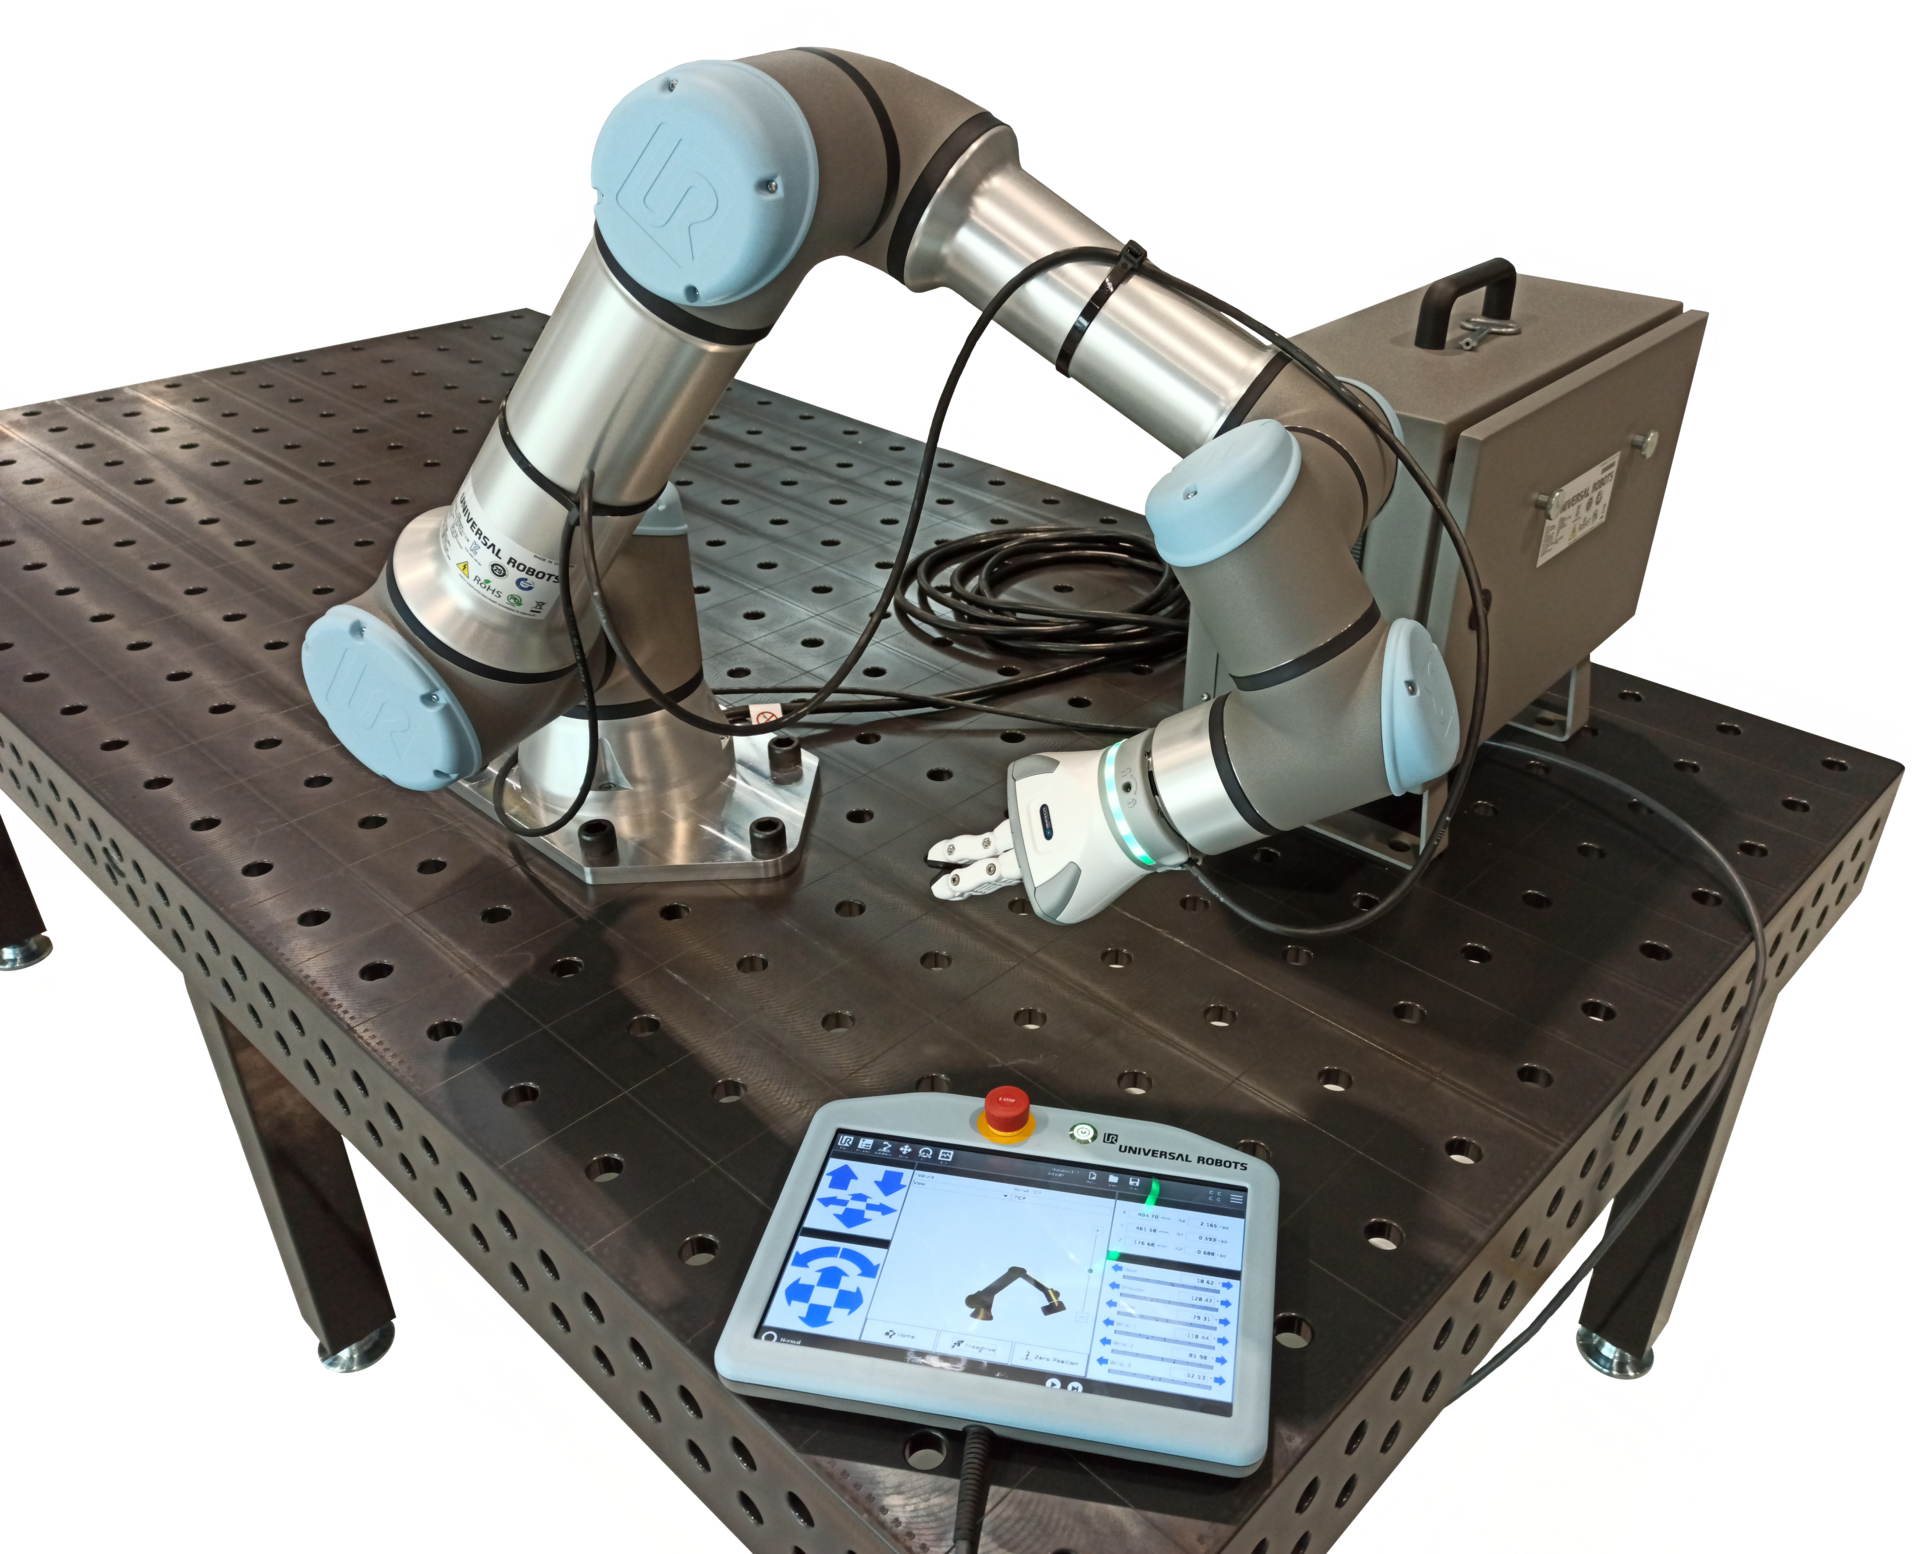
\includegraphics[width=\linewidth,height=3.8cm,keepaspectratio]{../../figures/r23_pendant.png}\\
\credit{Cobot arm with its teach pendant (front). Auledas, CC BY-SA 4.0, via Wikimedia Commons}
\column{.55\textwidth}
\begin{itemize}\small
\item Hand-held terminal: \term{jog} the robot, store points, edit and run programs.
\item \term{Jog modes}: joint by joint, or the tool along $x,y,z$ of a chosen frame.
\item \term{Enabling switch} (3 positions): robot moves only while held in the middle -- release \emph{or} squeeze hard $\to$ stop.
\item Manual mode \term{T1}: TCP speed limited to \hl{\SI{250}{mm/s}} (ISO 10218-1).
\item Emergency-stop button on every pendant.
\end{itemize}
\begin{keybox}[Teach workflow]
Jog to the point $\to$ check the tool angle $\to$ \textbf{store} the point $\to$ insert the move instruction $\to$ test slowly, step by step.
\end{keybox}
\end{columns}
\end{frame}

% ---------------------------------------------------------------------
\begin{frame}[t]{Coordinate frames: base, world, tool and user}
\begin{columns}[T,onlytextwidth]
\column{.52\textwidth}
\centering
\begin{tikzpicture}[x=1.15cm,y=1.15cm]
  \fill[mkLight] (-1,-.2) rectangle (5.4,0);
  \fill[mkBlue] (-.3,0) rectangle (.3,.35);
  \draw[mkBlue,line width=5pt,line cap=round] (0,.35) -- (.3,1.9) -- (2.2,2.5);
  \draw[mkMid,line width=3pt] (2.2,2.5) -- (2.6,2.0);
  \draw[mkGray,line width=2pt] (2.45,1.85) -- (2.75,2.15) (2.5,1.8) -- (2.4,1.6) (2.8,2.1) -- (2.95,1.95);
  \frm{(0,0)}{0}{base}{mkNavy}
  \frm{(2.68,1.72)}{-45}{tool}{mkOrange}
  \fill[mkPale,draw=mkMid] (3.0,0) -- (5.2,0) -- (5.2,.5) -- (3.0,.5) -- cycle;
  \frm{(3.1,.5)}{0}{user}{mkMid}
  \frm{(-.8,-1.0)}{0}{world}{mkGray}
  \node[font=\tiny,text=mkGray] at (4.1,.25) {fixture / table};
  \node[font=\tiny,text=mkOrange] at (3.6,1.9) {TCP};
\end{tikzpicture}
\column{.46\textwidth}
\begin{itemize}\small
\item \term{World}: the cell's fixed reference (useful with several robots).
\item \term{Base}: at the robot foot; the kinematics live here (4.3).
\item \term{Tool} (TCP frame): at the working point of the gripper or torch.
\item \term{User} / work-object: on the fixture or pallet.
\end{itemize}
\begin{notebox}
Every taught point is a pose: \textbf{tool frame relative to a user frame}. The controller chains the homogeneous transforms (4.2):
$T_\text{base}^\text{tool} = T_\text{base}^\text{user}\; T_\text{user}^\text{tool}$.
\end{notebox}
\end{columns}
\end{frame}

% ---------------------------------------------------------------------
\begin{frame}[t]{The tool frame (TCP) and why it must be right}
\begin{columns}[T,onlytextwidth]
\column{.48\textwidth}
\centering
\begin{tikzpicture}[x=1cm,y=1cm]
  \fill[mkOrange] (0,0) circle (.07); \node[font=\tiny,text=mkOrange,below] at (0,-.08) {fixed tip};
  \foreach \a/\c in {60/mkBlue,90/mkMid,120/mkSky,145/mkNavy}{
    \draw[\c,line width=3pt] (0,0) -- (\a:1.5); \fill[\c] (\a:1.5) circle (.12);}
  \node[font=\tiny,align=center,text=mkNavy] at (0,2.0) {4 different wrist orientations,\\same tip point};
\end{tikzpicture}
\begin{itemize}\small
\item \term{4-point method}: touch one fixed tip from 4 directions; the controller solves for the TCP offset.
\end{itemize}
\column{.5\textwidth}
\begin{itemize}\small
\item TCP = the point that moves along the programmed path and about which the tool rotates.
\item Wrong TCP $\to$ the tool ``wobbles'' when it re-orients.
\end{itemize}
\begin{defbox}[Worked example -- TCP error]
\footnotesize
\begin{enumerate}
\item TCP length error $e = \SI{5}{mm}$.
\item Re-orient the tool by $\theta = 30^\circ$ ``about the tip''.
\item Real tip moves on an arc: chord $= 2e\sin(\theta/2)$.
\item $= 2\cdot 5\cdot\sin 15^\circ = \hl{\SI{2.6}{mm}}$ -- a missed weld seam!
\end{enumerate}
\end{defbox}
\end{columns}
\end{frame}

% ---------------------------------------------------------------------
\begin{frame}[t]{User frames: teach once, move the fixture freely}
\begin{columns}[T,onlytextwidth]
\column{.48\textwidth}
\centering
\begin{tikzpicture}[x=.0055cm,y=.0055cm]
  \draw[mkGray,-{Latex}] (0,0) -- (1000,0) node[right,font=\tiny]{$x_b$};
  \draw[mkGray,-{Latex}] (0,0) -- (0,520) node[above,font=\tiny]{$y_b$};
  \node[font=\tiny,text=mkNavy,below left] at (0,0) {base};
  \fill[mkPale] (600,200) rectangle (850,450); \draw[mkMid] (600,200) rectangle (850,450);
  \draw[-{Latex},mkRed,thick] (800,200) -- (800,320) node[right,font=\tiny]{$x_u$};
  \draw[-{Latex},mkGreen,thick] (800,200) -- (680,200) node[below,font=\tiny]{$y_u$};
  \fill[mkMid] (800,200) circle (12) node[below right,font=\tiny]{O$_u$ (800, 200)};
  \fill[mkOrange] (750,300) circle (14) node[above,font=\tiny,text=mkOrange]{P};
  \foreach \x in {200,400,600,800}{\node[font=\tiny,text=mkGray,below] at (\x,0) {\x};}
\end{tikzpicture}
\begin{itemize}\small
\item Teach 3 points: origin, a point on $x_u$, a point in the $x_u y_u$ plane.
\end{itemize}
\column{.5\textwidth}
\begin{itemize}\small
\item Points are stored \hl{relative to the fixture}.
\item Fixture moved? Re-teach only its 3 frame points -- all 50 program points follow.
\end{itemize}
\begin{defbox}[Worked example]
\footnotesize
User frame: origin $(800,200)$ mm, rotated $90^\circ$ about $z$. Point P in user frame: $(100, 50)$ mm.
\begin{enumerate}
\item Rotate: $R(90^\circ)\,(100,50) = (-50, 100)$.
\item Add origin: $(800-50,\;200+100)$.
\item P in base frame $= \hl{(750, 300)}$ mm.
\end{enumerate}
\end{defbox}
\end{columns}
\end{frame}

% ---------------------------------------------------------------------
\begin{frame}[t]{Motion instructions: joint, linear, circular -- and blending}
\begin{columns}[T,onlytextwidth]
\column{.52\textwidth}
\centering
\begin{tikzpicture}[x=.85cm,y=.85cm]
  \foreach \p/\n in {(0,0)/P1,(2,2.2)/P2,(4.5,2.2)/P3,(5.5,0.4)/P4}{\fill[mkNavy] \p circle (.06); \node[font=\tiny,above] at \p {\n};}
  \draw[mkSky,thick,dashed] (0,0) .. controls (.2,1.6) and (1.2,2.3) .. (2,2.2);
  \node[font=\tiny,text=mkSky,anchor=east] at (.5,1.4) {MoveJ (curved, fast)};
  \draw[mkBlue,thick] (2,2.2) -- (3.9,2.2);
  \draw[mkOrange,thick] (3.9,2.2) .. controls (4.5,2.2) .. (4.75,1.75);
  \draw[mkBlue,thick] (4.75,1.75) -- (5.5,.4);
  \draw[mkOrange,dashed] (4.5,2.2) circle (.6);
  \node[font=\tiny,text=mkBlue] at (3,2.45) {MoveL (straight)};
  \node[font=\tiny,text=mkOrange,anchor=south] at (4.5,2.85) {zone: blend, no stop};
  \draw[mkMid,thick] (5.5,.4) arc (40:-120:.9);
  \node[font=\tiny,text=mkMid,anchor=west] at (5.0,-1.0) {MoveC (arc)};
\end{tikzpicture}
\column{.46\textwidth}
\begin{itemize}\small
\item \code{MoveJ}/PTP: joints interpolated; fastest, path not straight -- for free air moves.
\item \code{MoveL}: TCP on a straight line -- approach, welding, insertion.
\item \code{MoveC}: arc through an auxiliary point.
\item \term{Zone} / blending: pass \emph{near} a via-point without stopping $\to$ shorter cycle.
\end{itemize}
\begin{keybox}[Watch out]
MoveL can drive the arm through a \hl{singularity} (4.5); MoveJ cannot, but may swing wide.
\end{keybox}
\end{columns}
\end{frame}

% ---------------------------------------------------------------------
\begin{frame}[t]{A complete pick-and-place program (generic pseudo-code)}
\begin{columns}[T,onlytextwidth]
\column{.5\textwidth}
\begin{tcolorbox}[colback=mkLight,colframe=mkGray,boxrule=.4pt,arc=1mm,left=2mm,top=1mm,bottom=1mm]
\ttfamily\footnotesize
MoveJ Home, v1000, fine;\\
LOOP\\
\hspace*{1.1em}WaitDI PartReady = 1;\\
\hspace*{1.1em}MoveJ Offs(Pick,0,0,100), v1000, z50;\\
\hspace*{1.1em}MoveL Pick, v200, fine;\\
\hspace*{1.1em}SetDO Gripper = 1; Wait 0.2;\\
\hspace*{1.1em}MoveL Offs(Pick,0,0,100), v500, z20;\\
\hspace*{1.1em}MoveJ Offs(Place,0,0,100), v1000, z50;\\
\hspace*{1.1em}MoveL Place, v200, fine;\\
\hspace*{1.1em}SetDO Gripper = 0; Wait 0.2;\\
\hspace*{1.1em}MoveL Offs(Place,0,0,100), v500, z20;\\
\hspace*{1.1em}PulseDO Done;\\
ENDLOOP
\end{tcolorbox}
\column{.48\textwidth}
\begin{itemize}\small
\item \code{Offs(P,0,0,100)}: \SI{100}{mm} above P -- the \term{approach} point.
\item \code{v200}: speed in mm/s; \code{fine}: stop exactly; \code{z50}: blend with 50 mm zone.
\item \code{WaitDI}/\code{SetDO}: digital I/O -- the link to the PLC (5.4).
\item Only \hl{two points} (Pick, Place) need teaching; the rest is calculated.
\end{itemize}
\begin{notebox}
Pattern: approach fast in joint mode, last centimetres slowly and straight, act, retreat straight.
\end{notebox}
\end{columns}
\end{frame}

% ---------------------------------------------------------------------
\begin{frame}[t]{Variables and loops: one program, a whole pallet}
\begin{columns}[T,onlytextwidth]
\column{.46\textwidth}
\centering
\begin{tikzpicture}[x=1cm,y=1cm]
  \draw[mkGray,fill=mkLight] (-.2,-.2) rectangle (4.4,3.2);
  \foreach \i in {0,1,2,3}{\foreach \j in {0,1,2}{
    \draw[draw=mkBlue,fill=mkPale] (\i*1.05,\j*1.0) rectangle ++(1,.95);
    \node[font=\tiny,text=mkGray] at (\i*1.05+.5,\j*1.0+.47) {(\i,\j)};}}
  \fill[mkOrange,opacity=.5] (2*1.05,1.0) rectangle ++(1,.95);
  \draw[-{Latex},mkRed,thick] (0,0) -- (.8,0) node[below,font=\tiny]{$x$};
  \draw[-{Latex},mkGreen,thick] (0,0) -- (0,.8) node[left,font=\tiny]{$y$};
  \draw[{Latex}-{Latex},mkNavy] (0,-.45) -- (1.0,-.45) node[midway,below,font=\tiny]{$d_x$ = 400};
  \draw[{Latex}-{Latex},mkNavy] (4.6,0) -- (4.6,.95) node[midway,right,font=\tiny]{$d_y$ = 300};
\end{tikzpicture}\\
\footnotesize pallet user frame; boxes 400 $\times$ 300 $\times$ 200 mm
\column{.52\textwidth}
\begin{eqbox}\small
$P_{ijk} = P_0 + (i\,d_x,\; j\,d_y,\; k\,d_z)$
\end{eqbox}
\footnotesize $i$ = column, $j$ = row, $k$ = layer (counting from 0); $P_0$ = first box position.
\begin{defbox}[Worked example]
\footnotesize
\begin{enumerate}
\item $P_0 = (200, 150, 200)$ mm (centre of first box top).
\item Box $i=2$, $j=1$, layer $k=2$; $d_z = 200$ mm.
\item Offset $= (800, 300, 400)$ mm.
\item $P = \hl{(1000, 450, 600)}$ mm in the pallet frame.
\end{enumerate}
\end{defbox}
\small Three nested \code{FOR} loops place all $4\times3\times5 = 60$ boxes.
\end{columns}
\end{frame}

% ---------------------------------------------------------------------
\begin{frame}[t]{Offline programming (OLP): the workflow}
\centering
\begin{tikzpicture}[x=1cm,y=1cm]
  \foreach \i/\t/\s in {0/{CAD model\\of cell \& part}/blk,1/{generate\\paths}/blk,2/{simulate:\\reach, collision,\\cycle time}/blko,3/{post-process\\to robot\\language}/blk,4/{calibrate \&\\touch up on\\real cell}/blko}{
    \node[\s,minimum width=21mm,minimum height=12mm] (n\i) at (2.6*\i,0) {\t};}
  \foreach \a/\b in {0/1,1/2,2/3,3/4}{\draw[sig] (n\a) -- (n\b);}
  \draw[fb] (n2.south) -- ++(0,-.4) -| node[pos=.25,below,font=\tiny]{fix collisions / reach problems} (n1.south);
\end{tikzpicture}
\vspace{3mm}
\small
\begin{tabularx}{\linewidth}{@{}X X@{}}
\toprule
\textbf{Advantages} & \textbf{Challenges}\\
\midrule
No production stop while programming & Needs accurate models of robot, tools and cell\\
Test ideas and layouts before buying & Robot \emph{accuracy} (not repeatability) now matters\\
Complex paths from CAD (welding, deburring) & Cables, hoses and real part variation are not in CAD\\
\bottomrule
\end{tabularx}
\gofurther{Robot calibration identifies the real link lengths and joint offsets, cutting absolute error from about 1 mm to a few tenths of a mm.}
\end{frame}

% ---------------------------------------------------------------------
\begin{frame}[t]{Simulation: checking reach, collisions and cycle time}
\begin{columns}[T,onlytextwidth]
\column{.5\textwidth}
\begin{tikzpicture}
\begin{axis}[mkplot, width=6.8cm, height=4.6cm, xmin=0, xmax=8, ymin=-200, ymax=200,
  xlabel={time (s)}, ylabel={joint 5 angle (deg)}]
\addplot[mkBlue,thick,domain=0:8,samples=120] {120*sin(deg(0.9*x))+40*sin(deg(2.1*x))};
\addplot[mkRed,dashed,thick] coordinates {(0,120) (8,120)};
\addplot[mkRed,dashed,thick] coordinates {(0,-120) (8,-120)};
\node[font=\tiny,text=mkRed,anchor=south east] at (axis cs:8,122) {joint limit};
\end{axis}
\end{tikzpicture}
\column{.48\textwidth}
\begin{itemize}\small
\item \textbf{Reach \& orientation}: can the tool reach every point at the right angle?
\item \textbf{Joint limits \& singularities}: the plot shows joint 5 exceeding its limit $\to$ change the path or the part orientation.
\item \textbf{Collisions}: robot, tool, fence, machine.
\item \textbf{Cycle time}: realistic within a few \% if the controller model is good.
\end{itemize}
\begin{keybox}[Analogy]
A flight simulator for the robot: crash it on the computer, not in the cell.
\end{keybox}
\end{columns}
\end{frame}

% ---------------------------------------------------------------------
\begin{frame}[t]{From simulation to digital twin}
\begin{columns}[T,onlytextwidth]
\column{.52\textwidth}
\centering
\begin{tikzpicture}[x=1cm,y=1cm]
  \node[blk,minimum width=26mm,minimum height=14mm] (p) at (0,0) {\textbf{physical cell}\\robot, PLC, sensors};
  \node[blko,minimum width=26mm,minimum height=14mm] (v) at (4.4,0) {\textbf{virtual model}\\kinematics, logic,\\process};
  \draw[sig] ([yshift=3mm]p.east) -- node[above,font=\tiny]{live data (OPC UA, \ldots)} ([yshift=3mm]v.west);
  \draw[sig] ([yshift=-3mm]v.west) -- node[below,font=\tiny]{optimised programs, alarms} ([yshift=-3mm]p.west-|p.east);
  \node[font=\tiny,text=mkGray,align=center] at (2.2,-1.6) {model $\to$ (one-way) simulation;\\continuously synchronised $\to$ \hl{digital twin}};
\end{tikzpicture}
\column{.46\textwidth}
\begin{itemize}\small
\item \term{Virtual commissioning}: test the real PLC program against a simulated cell before installation.
\item \term{Digital twin}: model kept in sync with the real cell by live data.
\item Uses: predict cycle time, spot wear, try changes safely (Industry 4.0, 5.1).
\end{itemize}
\begin{notebox}
Virtual commissioning can move much of the on-site debugging to the office -- the real cell starts producing sooner.
\end{notebox}
\end{columns}
\end{frame}

% ---------------------------------------------------------------------
\begin{frame}[t]{Check your understanding -- 5.5}
\vspace{4mm}
\begin{keybox}[Check your understanding]
\large
\begin{enumerate}
\item A fixture is moved 50 mm. Why does a program written in a user frame need only 3 points re-taught?\\[3mm]
\item Which move type would you use to insert a pin into a hole -- and which to swing back to Home? Why?\\[3mm]
\item Give one reason why an offline program may miss the part on the real robot.
\end{enumerate}
\end{keybox}
\vfill
\centering\small\color{mkGray} Discuss with your neighbour for 3 minutes.
\end{frame}

% ---------------------------------------------------------------------
\begin{frame}{Summary 5.5 -- Robot programming}
\begin{columns}[T,onlytextwidth]
\column{.55\textwidth}
\begin{keybox}[Key take-aways]
\small
\begin{itemize}
\item Online (teach pendant, lead-through) vs.\ offline (OLP + simulation).
\item Frames: world, base, tool (TCP), user; points are stored relative to them.
\item Correct TCP and user frames make programs robust and portable.
\item MoveJ for free moves, MoveL/MoveC for process paths; zones save time.
\item Simulation checks reach, collisions, cycle time; a digital twin stays in sync.
\end{itemize}
\end{keybox}
\column{.42\textwidth}
\begin{defbox}[Key terms]
\small
\textbf{Teach pendant} -- hand-held programming unit.\\
\textbf{Jog} -- move the robot manually.\\
\textbf{TCP} -- tool centre point.\\
\textbf{User frame} -- frame on the work-piece.\\
\textbf{Zone} -- blend radius at a via-point.\\
\textbf{OLP} -- offline programming.
\end{defbox}
\end{columns}
\end{frame}

% =====================================================================
\section*{Wrap-up}
\begin{frame}[t]{Day summary}
\begin{columns}[T,onlytextwidth]
\column{.5\textwidth}
\centering
\begin{tikzpicture}[y=-.95cm]
  \foreach \y/\t/\c/\s in {0/{what robots do (applications)}/mkSky/5.2,1/{where they do it (the work-cell)}/mkMid/5.3,2/{who coordinates (the PLC)}/mkBlue/5.4,3/{how they are told (programming)}/mkOrange/5.5}{
    \node[draw=\c,fill=\c!15,rounded corners=2pt,minimum width=52mm,minimum height=7mm,font=\small,align=center] at (0,\y) {\t};
    \node[font=\scriptsize\bfseries,mkOrange] at (-3.1,\y) {\s};}
  \foreach \y in {0,1,2}{\draw[sig] (0,\y+.37) -- (0,\y+.63);}
\end{tikzpicture}
\column{.48\textwidth}
\begin{keybox}[Five things to remember]
\small
\begin{enumerate}
\item The process decides the robot (payload, path, speed).
\item Cycle time $\le$ takt time; check reach in the layout.
\item PLC: read -- execute -- write, every few ms.
\item Ladder: series AND, parallel OR, seal-in memory.
\item Teach points relative to good tool and user frames.
\end{enumerate}
\end{keybox}
\end{columns}
\end{frame}

% ---------------------------------------------------------------------
\begin{frame}[t]{Preview of Week 2 Day 4}
\begin{columns}[T,onlytextwidth]
\column{.55\textwidth}
\begin{defbox}[Tomorrow: manufacturing (cont.) and sensors I]
\small
\begin{itemize}
\item 5.6 Material handling: conveyors, AGV/AMR, FMS cells, cobots and human--robot collaboration.
\item 5.7 Safety and standards: risk assessment, ISO 10218, ISO/TS 15066, performance levels, light curtains, safety PLC.
\item 6.1--6.3 Sensors: accuracy and resolution; encoders, IMUs; force, proximity and range sensors.
\end{itemize}
\end{defbox}
\column{.42\textwidth}
\begin{keybox}[Think about it]
Today's cell had a fence. What would have to change for a person to work \emph{next to} the robot without one?
\end{keybox}
\end{columns}
\end{frame}

% ---------------------------------------------------------------------
\begin{frame}[t]{Figure credits}
\scriptsize
All plots, layouts, ladder diagrams, timing diagrams and schematics without a credit line are original drawings made for this course.
Downloaded figures (Wikimedia Commons):\\[2mm]
\begin{tabularx}{\linewidth}{@{}l X l@{}}
\toprule
\textbf{File} & \textbf{Source (Wikimedia Commons) and author} & \textbf{Licence}\\
\midrule
r23\_spot\_welding.jpg & File:BMW Leipzig MEDIA 050719 Download Karosseriebau max.jpg -- BMW Werk Leipzig & CC BY-SA 2.0 de\\
r23\_painting.jpg & File:Japan- Painting Robot.jpg -- Gary Todd & CC0\\
r23\_palletising.jpg & File:Factory Automation Robotics Palettizing Bread.jpg -- KUKA Roboter GmbH, Bachmann & Public domain\\
r23\_delta.jpg & File:Delta x robot - vision module - conveyor.jpg -- Trungdoanhong & CC BY-SA 4.0\\
r23\_plc.jpg & File:S71500.JPG -- Palatinatian & CC BY 3.0\\
r23\_pendant.png & File:UR16e robot arm.png -- Auledas & CC BY-SA 4.0\\
\bottomrule
\end{tabularx}
\end{frame}

% ---------------------------------------------------------------------
\begin{frame}[t]{References}
\fontsize{6}{7}\selectfont\setlength{\itemsep}{0pt}
\begin{columns}[T,onlytextwidth]
\column{.5\textwidth}
\begin{itemize}
\item Groover, M.\,P.: \emph{Automation, Production Systems, and Computer-Integrated Manufacturing}, 4th ed. Pearson, 2015.
\item Nof, S.\,Y. (ed.): \emph{Handbook of Industrial Robotics}, 2nd ed. Wiley, 1999.
\item Siciliano, B.; Khatib, O. (eds.): \emph{Springer Handbook of Robotics}, 2nd ed. Springer, 2016.
\item Craig, J.\,J.: \emph{Introduction to Robotics: Mechanics and Control}, 4th ed. Pearson, 2018.
\item Boothroyd, G.: \emph{Assembly Automation and Product Design}, 2nd ed. CRC Press, 2005.
\item Whitney, D.\,E.: \emph{Mechanical Assemblies}. Oxford Univ.\ Press, 2004.
\item International Federation of Robotics: \emph{World Robotics -- Industrial Robots} (annual report).
\item Pan, Z.\ et al.: Recent progress on programming methods for industrial robots. \emph{Robotics and Computer-Integrated Manufacturing} 28(2), 2012.
\end{itemize}
\column{.48\textwidth}
\begin{itemize}
\item Bolton, W.: \emph{Programmable Logic Controllers}, 6th ed. Newnes, 2015.
\item Petruzella, F.\,D.: \emph{Programmable Logic Controllers}, 5th ed. McGraw-Hill, 2016.
\item John, K.-H.; Tiegelkamp, M.: \emph{IEC 61131-3: Programming Industrial Automation Systems}, 2nd ed. Springer, 2010.
\item IEC 61131-3:2013 Programmable controllers -- Part 3: Programming languages.
\item ISO 9283:1998 Manipulating industrial robots -- Performance criteria and related test methods.
\item ISO 9787:2013 Robots and robotic devices -- Coordinate systems and motion nomenclatures.
\item ISO 10218-1:2011 Robots and robotic devices -- Safety requirements for industrial robots -- Part 1: Robots.
\item Grieves, M.; Vickers, J.: Digital twin: mitigating unpredictable, undesirable emergent behavior in complex systems. In \emph{Transdisciplinary Perspectives on Complex Systems}, Springer, 2017.
\end{itemize}
\end{columns}
\end{frame}

\end{document}
